%!TEX encoding = UTF-8 Unicode
%!TEX program = xelatex

\documentclass[master]{ustcthesis}
% bachelor|master|doctor

%\hypersetup{colorlinks=false}  %打印版去掉该注释,链接变黑色
\usepackage{ustcextra}
\usepackage{physics}
\usepackage{bm}
\usepackage{float}



\graphicspath{{figures/}{figures/chap1/}{figures/chap2}
    {figures/chap3}{figures/chap4}{figures/chap5}{figures/chap6}}

\DeclareMathOperator\erfc{erfc}
\DeclareMathOperator\E{E}
\DeclareMathOperator\Var{Var}



    
    
\title{光通信中量子接收机的理论研究与实验平台搭建}
\author{左元}
\major{电磁场与微波技术}
\advisor{朱 冰\ 教授}
\submitdate{二〇一六年五月}
%\secrettext{机密\quad 小于等于20年}   % 内部|秘密|机密,注释本行则不保密
\depart{06系}

\entitle{Theory Analysis of Quantum Receivers in Optical Communication System and Experimental Platform Building}
\enauthor{Yuan Zuo}
\enmajor{Electromagnetic Field and \\ \hspace*{8.7cm}\hfill Microwave Technology}
\enadvisor{Prof. Bing Zhu}
\ensubmitdate{May, 2016}
%\ensecrettext{Confidential\quad Less than or equal to 20 years}  % Internal|Secret|Confidential

\begin{document}

\maketitle

%
% 本科论文:
%   frontmatter: 致谢、目录、中文摘要、英文摘要
%   mainmatter: 正文章节、参考文献
%   appendix: 附录
%
% 硕博论文:
%   frontmatter: 中文摘要、英文摘要、目录、符号说明
%   mainmatter: 正文、参考文献
%   appendix: 附录
%   backmatter: 致谢、发表论文
%

\frontmatter
\begin{abstract}
在经典光通信系统中,由于受到散粒噪声的影响,
通信系统接收机性能存在着经典极限——标准量子极限(standard quantum limit, SQL)。
近年来,随着量子信息技术的发展,利用光的量子特性设计新型的光接收机方案逐渐引起学术界的关注。
这是因为,采用量子探测和测量的技术可以获取之前使用经典探测所不能获得的信息。
这种方案可以让系统的性能突破标准量子极限,
从而获得经典检测方案所不能达到的更低的误码率和更高的信道容量。
当前对量子接收机的研究进展还比较缓慢,尚停留在理论研究和初步实验验证阶段,
仍然有许多值得研究的理论和实验课题。


在本论文中,我们首先回顾一下自上个世纪六十年代量子接收机只提出以来的研究进展,
然后就以下三个问题进行深入探究:


1. QAM信号量子接收机理论研究。
到目前为止,二元调制和相位调制(PSK)方案的量子接收机,
国际上已经有较多的研究人员关注,也取得了很多具有突破意义
的成果。但是对于更高阶调制的QAM信号,研究人员关注的还较少。
本文将目前几种接收机方案推广到QAM信号,对QAM信号的量子接收机
进行系统的研究。这些接收机包括Bondurant接收机、
自适应分区检测接收机和混合接收机等三种接收机方案。
通过对三种接收机方案进行对比,可以为工程上可实现的量子接收机方案设计
提供参考。

2. 二元调制多符号信号条件归零接收机理论研究。
相比于对单个符号的检测方案,采用联合检测思想的条件归零接收机
更具有研究价值。在本文中,我们将条件归零接收机的方案
应用到多脉冲脉冲位置调制(MPPM)、编码后的OOK调制、
编码后的BPSK调制信号。在此基础上,通过对接收机接收策略的优化,
我们将接收机的误码率降低到经典检测方案的标准量子极限以下。

3. 量子接收机初步实验研究。
作为初步实验验证工作,本文对BPSK的Kennedy接收机,进行初步的实验验证工作。
实验结果表明,在相同的系统效率的情况下,我们的Kennedy接收机性能能够突破标准量子极限。
通过替换发射端的态制备光调制器和接收端的光调制器,
原则上这种方案可以用于任意PSK信号的量子接收机的实验研究。







\keywords{量子接收机\zhspace 标准量子极限\zhspace QAM调制\zhspace 
量子编码\zhspace 光通信}

\end{abstract}


\begin{enabstract}
In the classical optical communication systems, 
due to the influence of shot noise,
the receiver performances of the communication system  
are limited by the standard quantum limit (SQL).
In recent years, with the development of quantum information technology, 
the optical receivers using quantum properties of light 
are concerned by researchers.
Because the quantum detection and measurement  technology can extract the information 
that not be obtained by classical measurement methods.
It enables the performance of the system outperforming the standard quantum limit,
and achieving lower bit error rate and higher channel capacity than classic detection schemes.
Nowadays research progress on quantum receivers is still relatively slow. 
It stays in the theoretical study and experimental demonstration stage,
There are still many theoretical and experimental problems worthy of study.


In this paper, we first review the research progress since the 1960's when the quantum receivers were proposed ,
then focus on following three issues:


1. The theory of quantum receiver for QAM signals.
So far, quantum receiver for binary modulation signals and phase modulation (PSK) signals 
have been deeply studied, and a lot of breakthrough have been work out.
But for higher order modulation such as QAM signals, the researchers are careless.
This article will present several receivers for the QAM signals and compare these three receivers.
These receivers include a  Bondurant receiver, 
adaptive partitioning detection receiver and hybrid receivers.
By comparing three receivers, some information can be applied to 
design engineering achievable quantum receiver scheme for reference.

2. Theoretical study of conditional nulling receivers for binary modulation multi-symbol signals.
Compared to a single symbol detection scheme, conditional nulling receivers using joint detection  
are more valuable to research. In this article, we will applied the conditional nulling receiver schemes
to the multi-pulse pulse position modulation (MPPM), coding OOK modulation signals,
coding BPSK modulation signals. On this basis, through optimizing the receive policy,
the error probabilities of the receivers are reduced below the SQL of the classic detection scheme.

3. Initial experiment research of  the quantum receivers .
As an initial experimently demostration work, we implement the Kennedy BPSK receiver in this paper 
to preliminary validate the Kennedy receiver theory.
Experiment results show that our Kenendy receiver can outperform the SQL in the same system effiency codition.
By replace the modulator in the phase of the preparation stage and the receive stage,
such receiver can, in principle, be applied to arbitrary PSK signals.

\enkeywords{quantum receiver, standard quantum limit, QAM modulation, quantum code, optical communication}
\end{enabstract}

{\hypersetup{linkcolor=black}
\tableofcontents
\listoffigures
%\listoftables
}

%\listofalgorithms  % 算法索引,如不需要,可直接注释掉本行
%\lstlistoflistings % 代码索引。添加代码索引,会导致PDF书签中目录出现两次,故暂不添加
% \begin{notation}

\centering
\begin{tabular}{rl}
$\ln x$ & natural logarithm $\log_ex$ \\
$\log x$ & common logarithm $\log_{10}x$ \\
$x\ \mathrm{mod}\ y$ & remainder \\
\end{tabular}

\end{notation}


\mainmatter
\chapter{绪论}
\section{研究背景简介}

\subsection{量子信息技术简介}

\subsection{量子接收机的国内外研究现状}




\section{论文主要内容}

\chapter{量子光通信的理论基础}

\section{电磁场的量子态描述}
\subsection{相干态}
通信中常用相干光来传递信息,在数学上,它可以用一个正弦波来表示。
在物理实现上,它可以用线偏振的电场来实现\cite{djordjevic2010fundamentals},
\begin{equation}
\bm{E}(t) = \bm{p} A e^{j\omega t + \phi}.
\end{equation}
上式中,符号$\bm{p}$、$A$、$\omega$和$\phi$分别对应偏振矢量、幅度、频率和相位。
要传递的信息被调制在场的这四个要素上面。
在本文中,主要关注的是对幅度和相位的调制。
这两个要素可以用一个复振幅来描述
\begin{equation}
\alpha = A e^{j\phi}.
\end{equation}
该复振幅也可以用相空间复平面中的一个点来表示,这种相空间图像被称作星座图。
图\ref{fig:signals}展示了OOK、BPSK、QPSK、16-QAM四种常见的调制信号的星座图。

\begin{figure}
\centering
  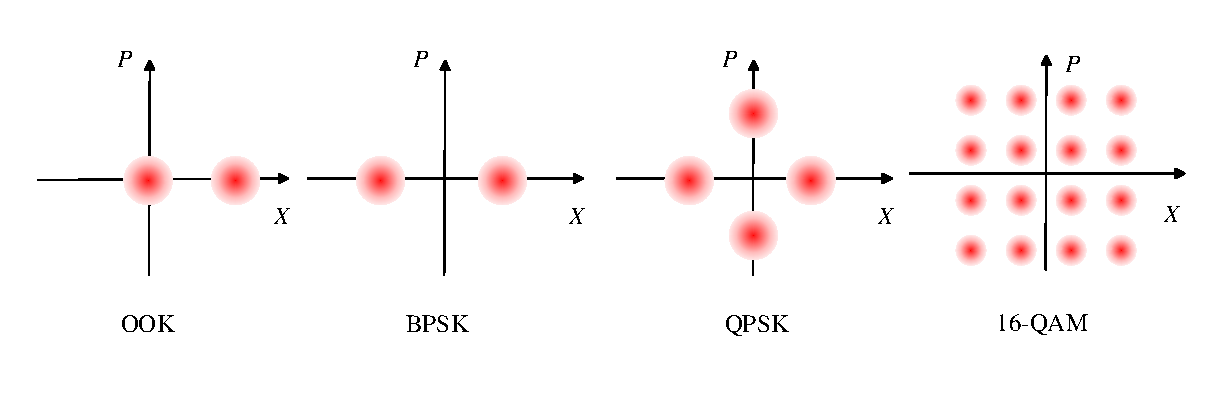
\includegraphics[width=\textwidth]{figures/chap2/signals}
  \caption{常见的四种调制信号星座图}
  \label{fig:signals}
\end{figure}

在量子力学中,电磁场被量子化为若干个不同模式、不同频率的光子\cite{gerry2005introductory,helstrom1976quantum,mandel1995optical}。
单模电磁场的哈密顿量可以表示为无穷个Fork态的线性叠加
\begin{equation}
\hat{H} = \hbar \omega (\hat{a}^\dagger \hat{a} + \frac{1}{2}).
\end{equation}
其中$\hat{a}^\dagger$和 $\hat{a}$ 分别是产生算符和湮灭算符,
乘积$\hat{a}^\dagger \hat{a}$是粒子数算符,他的本振态是Fork态$\ket{n}$,满足
\begin{equation}
\hat{a}^\dagger \hat{a} \ket{n} = n \ket{n}.
\end{equation}

通信中常用的单模相干光脉冲可以用单模相干态$\ket{\alpha}$来描述,它是湮灭算符的本振态
\begin{equation}
\hat{a} \ket{\alpha} = \alpha \ket{\alpha}.
\end{equation}
在Fork态表象中,相干态可以表达为
\begin{equation}
\ket{\alpha} = \exp(-\frac{1}{2}|\alpha|^2) \sum_{n=0}^\infty \frac{\alpha^n}{\sqrt{n!}} \ket{n}.
\end{equation}
如果用光子计数器进行探测,相干态$\ket{\alpha}$探测到的光子数不是一个固定的值,
而是服从泊松分布
\begin{equation}
P_n = |\bra{n}\ket{\alpha}|^2 = \exp(-|\alpha|^2) \frac{|\alpha|^{2n}}{n!} .
\end{equation}
它的平均光子数由
\begin{equation}
\bar{n} = |\alpha|^2
\end{equation}
给出。相干态参数${\alpha}$可以是任何复数,具有复振幅的意义\cite{glauber1963coherent}。

任意两个相干态互不正交,两个相干态的内积为
\begin{equation}
\begin{split}
\bra{\alpha}\ket{\beta} &= \exp(-\frac{1}{2}|\alpha|^2 - \frac{1}{2} |\beta|^2) \sum_{n=0}^\infty \frac{(\alpha^*\beta)^n}{n!} \\
                         &= \exp(\alpha^*\beta -\frac{1}{2}|\alpha|^2 - \frac{1}{2} |\beta|^2).
\end{split}
\end{equation}
恒大于0。相干态互不正交是使得相干态无法完美区分的关键原因。

数学上也常常用密度矩阵来表示信号\cite{wt2001qm},相干态$\ket{\alpha}$也可以用密度矩阵表示为
$\hat{\rho} = \ket{\alpha}\bra{\alpha}$。



\subsection{位移操作}

\begin{figure}
\centering
  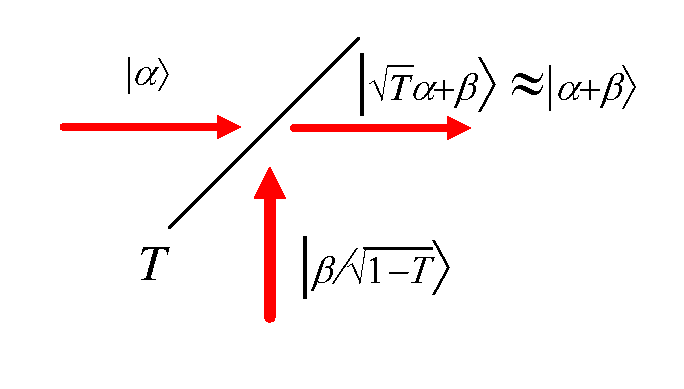
\includegraphics[height=5cm]{figures/chap2/displacement-operator}
  \caption{用波束分束器实现位移操作示意图}
  \label{fig:diaplacement}
\end{figure}

相干态可以通过位移操作进行变换,位移算符定义为\cite{glauber1963coherent,gerry2005introductory,helstrom1976quantum,mandel1995optical}
\begin{equation}
\hat{D}(\alpha) = \exp(\alpha \hat{a}^\dagger - \alpha^* \hat{a}).
\end{equation}
利用位移算符,相干态可以通过对真空态$\ket{0}$位移得到
\begin{equation}
\ket{\alpha} = \hat{D}(\alpha) \ket{0}.
\end{equation}
两个相干态之间也可以通过位移操作进行变换
\begin{equation}
\hat{D}(\beta) \ket{\alpha} = \ket{\alpha + \beta} .
\end{equation}


在实验当中,常用一个相位稳定干涉仪或者波束分束器来实现对相干态的位移操作\cite{cook2007optical,becerra2013experimental,lau2006binary,paris1996displacement}。
图\ref{fig:diaplacement}显示的是利用一个高透过率的波束分束器,
将两个入射场混合输出,近似实现了对其中一个入射场的位移操作,
这种方案在量子接收机实验中经常见到。

\section{经典光通信的接收方案}

在经典光通信中,有三类常见的接收方案,他们分别是
直接检测、零差接收和外差接收。
这三种接收方案受散粒噪声的制约,
使得每一种接收方案存在一个经典极限
——标准量子极限(Standard Quantum Limit)。
接下来,我们简单介绍一下每一种接收方案的具体实现方案。

\subsection{直接检测}



\begin{figure}
\centering
  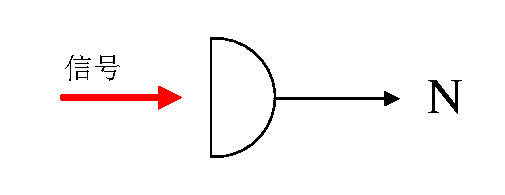
\includegraphics[scale=1]{figures/chap2/DD.pdf}
  \caption{直接检测示意图}
  \label{fig:DD}
\end{figure}


在所有的调制方案中,有一类采用脉冲的有无对信息进行编码,
比如开关键控(OOK)和脉冲位置调制(PPM)。
OOK调制将符号0编码为没有光脉冲,
而将符号1编码为有脉冲;PPM调制则将信息编码到脉冲所在的位置上。
对于这样一类的调制方案,经典光通信中常采用直接检测方案进行探测。
如图\ref{fig:DD}所示,直接检测方案直接探测信号光的强度,
来判断是否存在光脉冲或者光脉冲的幅度\cite{gagliardi1976optical,gagliardi1998optical}。
这种方案可以利用一个光电探测器或单光子探测器实现。
探测器可以输出探测到的光子数目,理想情况下,
对于给定的相干态,探测到$n$个光子的概率
\begin{equation}
\Pr(N = n| \ket{\alpha}) = \frac{|\alpha|^{2n}}{n!} e^{-|\alpha|^2}
\label{eq:dd-prob}
\end{equation}
一般地,对于信号矢态为$\ket{\phi}$的情况下,检测概率为
\begin{equation}
\Pr(N = n| \ket{\phi}) = |\bra{n}\ket{\phi}|^2
\end{equation}



\subsection{零差接收}
零差接收机是一种相干检测方案,如图\ref{fig:HD}所示,
是一种平衡零差接收方案\cite{gagliardi1976optical,gagliardi1998optical}。
这种接收方案和直接检测不同的是,
需要一个本振。对于零差接收本振频率和信号频率一致。
通常本振强度$a_{LO}$远大于信号强度$a_S$,
两路信号通过一个50:50的分束器,
在两个输出口得到两路新的信号$a_+$和$a_-$,满足关系式
\begin{equation}
a_\pm = \frac{a_S \pm a_{LO}}{\sqrt{2}}.
\end{equation}
这两路信号被光电探测器接收,得到两路光电流$i_\pm$。
这两路电流通过一个放大系数为$1/K=1/2q\sqrt{N_{LO}}$的差分放大器,
最后通过一个低通滤波器积分得到输出统计量
\begin{equation}
\alpha_\theta = \frac{N_+ - N_-}{2\sqrt{N_{LO}}}.
\end{equation}
这里假定所有的器件都是理想的。当$N_{LO} \rightarrow \infty$时,
输出统计量服从高斯分布
\begin{equation}
\alpha_\theta \sim N(\Re(ae^{-j\theta}), \frac{1}{4}).
\label{eq:HD-alpha}
\end{equation}
其中$\theta$是本振与信号的相位差。
这种测量方案,用量子力学算符可以用湮灭算符描述为\cite{yuen1980optical,mandel1995optical}
\begin{equation}
\hat{\alpha}_\theta = \Re(\hat{a}_S e^{-j\theta}).
\end{equation}


\begin{figure}
\centering
  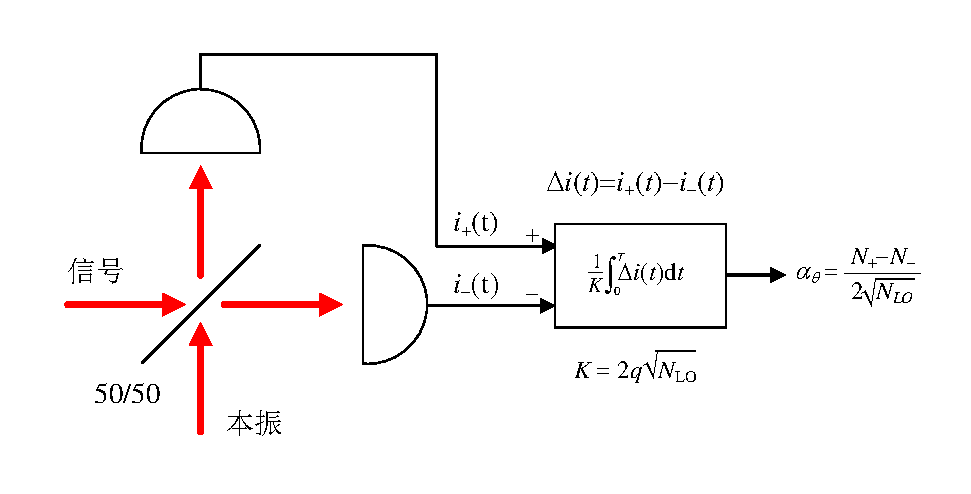
\includegraphics[width=0.8\textwidth]{figures/chap2/homodyne-receiver.pdf}
  \caption{平衡零差检测示意图}
  \label{fig:HD}
\end{figure}

\subsection{外差接收}
在上一小节,我们已经介绍了零差接收方案。
另外一种相干接收方案是外差接收\cite{gagliardi1976optical,gagliardi1998optical},
它采用了与信号频率不同的本振。
图\ref{fig:HeD}是一种平衡外差接收机示意图,
在这种外差接收机中,频率为$\omega$的信号场$a_S$
与频率为$\omega - \omega_{IF}$的强本振场$a_{LO}$
通过一个50:50的分束器混合。
混合后经过光电探测器,得到两路以中频$\omega_{IF}$震荡的电流$i_\pm$。
这两路电流经过一个放大系数为$1/K'=1/q\sqrt{N_{LO}}$的差分放大器,
最后解调出两个正交幅度$\alpha_1$和$\alpha_2$。
假定所有的器件都是理想的,当$N_{LO} \rightarrow \infty$时,
这两个统计量统计独立,分别服从高斯分布
\begin{equation}
\alpha_i \sim N(a_{S_i}, \frac{1}{2}).
\label{eq:Her-receiver-output}
\end{equation}
其中$a_{S_1}=\Re(a_S)$和$a_{S_2}=\Im(a_S)$分别是信号场的两个正交幅度。
这种测量方案,同时测量信号的两个正交幅度,
用量子力学算符湮灭算符可以描述为\cite{yuen1980optical,mandel1995optical}
\begin{equation}
\hat{\alpha}_1 + j \hat{\alpha}_2 = \hat{a}_S.
\label{eq:Her-receiver-output-2}
\end{equation}



\begin{figure}
\centering
  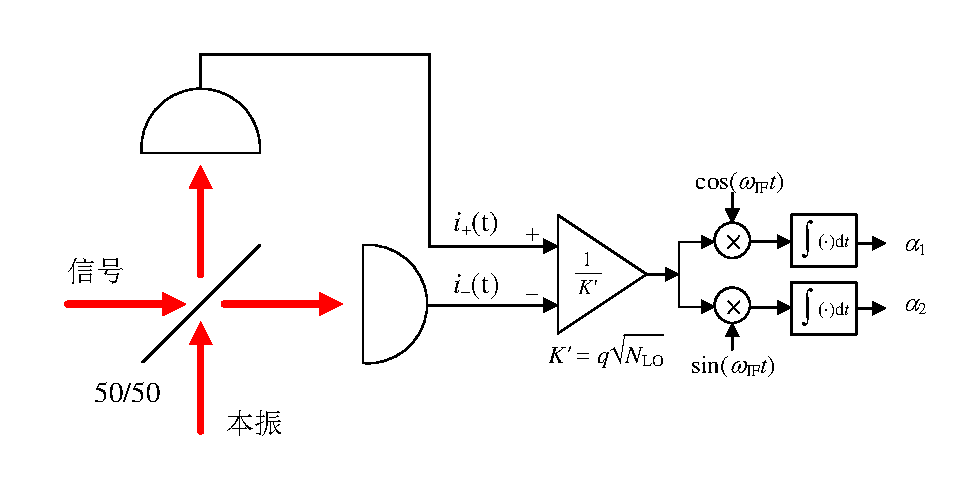
\includegraphics[width=0.8\textwidth]{figures/chap2/heretrodyne-receiver.pdf}
  \caption{平衡外差检测示意图}
  \label{fig:HeD}
\end{figure}


\section{量子检测与估计理论}
\subsection{经典最优检测}
通信系统通常由发送端、信道和接收端三个部分组成。
对某种特定的通信方案,发送端从$M$个符号中以先验概率分布$\zeta_j(j=1,2,...,M)$选择一个发送出去。
先验概率满足归一化条件
\begin{equation}
\sum_{j=1}^M \zeta_j = 1.
\end{equation}
我们称一个假设$H_j (j=1,2,...,M)$是指发送的是第$j$个符号。



在通信的接收端,接收机对电磁场进行探测,可以得到一些统计量。
例如在前面介绍的三种经典监测方案,输出的统计量分别是光子数目、
$\alpha_\theta$、$\{\alpha_1, \alpha_2\}$。
由于量子涨落和噪声的影响,对于给定的发送信号,
这些统计量通常不是一个固定的值,而是一个随机变量。
一般的,我们假设输出统计量是一个实随机向量$\bm{v} = (v_1, v_2, ..., v_n)$。
当发送第$j$个符号时,
假定它的联合分布为
$p_j(\bm{v}) = p_j(v_1, v_2, ..., v_n)$。
在通信的接收端,通过对接收到的统计量进行判决,
判定发送的符号是哪一个。
下面介绍两种重要的准则——贝叶斯准则和最小错误概率准则。

我们定义决策代价$C_{ij}$为,
当假设$H_j$是正确的情况下,选择了假设$H_i$所需要的代价。
我们期望一个决策是最优的是指该决策所需要的平均代价最小。

我们再来将决策数学化\cite{yzf2002tjxhcl,helstrom1976quantum},
定义在观测到的统计量为$\bm{v}$时,
选择了假设$H_i$的概率为$\pi_i(\bm{v})$,$i=1,2,...,M$。
这些决策概率需满足条件
\begin{equation}
0 \le \pi_i(\bm{v}) \le 1,  \sum_{i=1}^M \pi_i(\bm{v}) = 1.
\label{eq:pi-cond}
\end{equation}
一个简单的例子是一种被称为随机策略的决策方案,
对于任意观测量,这种策略都是随机选择一个假设,
即$\pi_i(\bm{v}) \equiv 1/M, \forall i, \bm{v}$。

在上述符号的约定下,我们可以得到在假设$H_j$是正确的情况下,
策略选择了假设$H_i$的条件概率为
\begin{equation}
\Pr\{i|j\} = \int_{\mathbb{R}^n} \pi_i(\bm{v}) p_j(\bm{v}) d^n \bm{v}.
\end{equation}
这里$\mathbb{R}$代表实数集合,$\mathbb{R}^n$代表$n$维实欧几里得空间。
那么,对所有的观测结果,平均代价为
\begin{equation}
\begin{split}
\bar{C} &= \sum_{i=1}^M \sum_{j=1}^M \zeta_j C_{ij} \Pr{i|j} \\
 &= \sum_{i=1}^M \sum_{j=1}^M \zeta_j C_{ij} \int_{\mathbb{R}^n} \pi_i(\bm{v}) p_j(\bm{v}) d^n \bm{v}.
\end{split}
\end{equation}
对于每一个假设$H_i$,我们定义它的风险函数
\begin{equation}
W_i(\bm{v}) = \sum_{j=1}^M \zeta_j C_{ij} p_j(\bm{v})。
\end{equation}
那么决策的平均代价可以改写为
\begin{equation}
\bar{C} =  \int_{\mathbb{R}^n} \sum_{i=1}^M W_i(\bm{v}) \pi_i(\bm{v}) d^n \bm{v}.
\label{eq:avg-C}
\end{equation}

在式\ref{eq:pi-cond}条件下,最小化式\ref{eq:avg-C},
这是一个凸优化问题。
这个问题可以通过一个简单的观察得以解决。
从式\ref{eq:pi-cond}和\ref{eq:avg-C}可以看出,
对于每一个观测结果$\bm{v} \in \mathbb{R}^n $,要使得平均代价最小,
需要选择风险$W_i(\bm{v})$最小的那一个假设。
即对于每一个观测结果$\bm{v} \in \mathbb{R}^n $,若
\begin{equation}
W_j(\bm{v}) < W_i(\bm{v}), \forall i \neq j,
\end{equation}
那么
\begin{equation}
\pi_j(\bm{v})=1, \pi_i(\bm{v}) \equiv 0, \forall i \neq j.
\end{equation}

为方便记函数
\begin{equation}
\Upsilon(\bm{v}) = \min_j W_j(\bm{v}), 
\end{equation}
那么对所有的观测结果$\bm{v}$和所有的假设$H_i$,有下式成立
\begin{equation}
\begin{split}
[W_i(\bm{v}) - \Upsilon(\bm{v})] \pi_i(\bm{v}) &= 0,  \\
W_i(\bm{v}) - \Upsilon(\bm{v}) &\ge 0.
\label{eq:classic-opt-cond}
\end{split}
\end{equation}
对式\ref{eq:classic-opt-cond}的第一个式子求和,可以得到
\begin{equation}
\Upsilon(\bm{v}) = \sum_i^M W_i(\bm{v})\pi_i(\bm{v}), 
\end{equation}
因此,可以得到最小平均代价为
\begin{equation}
\bar{C}_{min} = \int_{\mathbb{R}^n} \Upsilon(\bm{v}) d^n \bm{v}. 
\end{equation}
容易验证,这样得到的平均代价确实是最小平均代价,
即对任意其他的决策函数$\{\pi_i'(\bm{v})\}$,有
\begin{equation}
\bar{C}' - \bar{C}_{min} = \sum_{i=1}^M \int_{\mathbb{R}^n} [W_i(\bm{v}) - \Upsilon] \pi_i'(\bm{v}) d^n \bm{v} \ge 0. 
\end{equation}


现代的文献中,常将这种最小化平均代价函数的决策称作贝叶斯准则。
在这当中,有一种被称为最小错误概率准则的策略,它的决策代价系数定义为
\begin{equation}
C_{ii} = -1; C_{ij}=0, \forall i\neq j. 
\label{eq:min-err-cond}
\end{equation}
在这种决策代价下,最小平均代价就是最小平均错误概率
\begin{equation}
P_e = 1 - \sum_{j=1}^M \zeta_j \Pr{j|j} = \sum_{j=1}^M \zeta_j \sum_{k\neq j}\Pr{k|j}.
\end{equation}
在通信中,常用最小平均错误概率准则来设计接收机的接收策略。
因此本文也主要以该准则来设计量子接收机。

通过经典的三种探测方式加上经典检测预估计理论所得到的最佳接收方案,
它能达到的最小平均错误概率通常被称作标准量子极限(SQL)。




\subsection{量子最优检测}
上世纪六十年代,C.W. Helstrom和H. P. Yuen等人
将假设检验理论与量子力学结合起来,
发展出一套适用于量子测量的量子检测与估计理论
\cite{helstrom1976quantum,helstrom1967detection,yuen1975optimum}。
根据这一套理论,可以从理论上给出最优检测的数学形式,
下面我们简单回顾一下这个理论的主要内容。

在量子力学中,一个测量在数学上被描述为一个正定算子值测量(POVM)算符\cite{helstrom1976quantum}。
如果用算符$\hat{\Pi}_i (i=1,2,...,M)$表示一组POVM测量,
那么一组完备的POVM测量需要满足条件
\begin{equation}
\begin{split}
\hat{\Pi}_i & \ge 0, \\
\sum_{i=1}^M \hat{\Pi}_i & = \hat{I}.
\end{split}
\end{equation}

例如,直接检测利用POVM算符可以表达为
\begin{equation}
\hat{\Pi}_n = \ket{n}\bra{n}, n=0,1,2,...
\end{equation}
其中$\ket{n}$是Fork态矢量,这是一组正交投影测量。
我们说一组测量是正交投影测量是指它们满足正交条件
\begin{equation}
\hat{\Pi}_i \hat{\Pi}_j = 0, \forall i \neq j
\end{equation}
和投影算符条件
\begin{equation}
\hat{\Pi}_n^2 = \hat{\Pi}_n, n=0,1,2,...
\end{equation}
如果直接检测采用ON-OFF探测器,即只能探测到有光子还是没有光子,
那么直接检测对应于一个二元测量
\begin{equation}
\hat{\Pi}_0 = \ket{0}\bra{0}, \hat{\Pi}_1 = \hat{I} - \ket{0}\bra{0}.
\end{equation}


假设发送的信号态用密度矩阵为$\hat{\rho}_j$,那么将符号$j$检测为符号$i$的条件概率为
\begin{equation}
\Pr(i|j) = \Tr(\hat{\rho}_j \hat{\Pi}_i), (i,j)=1,2,...,M.
\end{equation}
那么利用上一节的符号定义,在这样的信号和测量设置下,
总的平均代价为
\begin{equation}
\bar{C} =  \sum_{i=1}^M \sum_{j=1}^M \zeta_jC_{ij} \Tr(\hat{\rho}_j \hat{\Pi}_i) \\
        =  \Tr \sum_{i=1}^M \hat{W}_i \hat{\Pi}_i.
\label{eq:q-avg-C}
\end{equation}
这里,风险算符$\hat{W}_i$定义为
\begin{equation}
\hat{W}_i = \sum_{j=1}^M \zeta_jC_{ij}\hat{\rho}_j.
\end{equation}
这样,我们得到与经典检测理论对应的优化问题。
H. P. Yuen和C. W. Helstrom等人给出该优化问题的一个充要条件,
\begin{equation}
\begin{split}
(\hat{W}_i - \hat{\Upsilon})\hat{\Pi}_i = \hat{\Pi}_i(\hat{W}_i - \hat{\Upsilon}) & = \bm{0}, i=1,2,...,M,  \\
\hat{W}_i - \hat{\Upsilon} & \ge \bm{0}, i=1,2,...,M.
\label{eq:optim-povm-cond}
\end{split}
\end{equation}
其中拉格朗日算符
\begin{equation}
\hat{\Upsilon} = \sum_{j=1}^M \hat{\Pi}_j\hat{W}_j = \sum_{j=1}^M\hat{W}_j\hat{\Pi}_j.
\end{equation}
那么,最小平均代价可以简化为
\begin{equation}
\bar{C}_{min} = \Tr(\hat{\Upsilon}).
\end{equation}

若取式\ref{eq:min-err-cond}中的最小平均错误概率准则决策代价系数,
那么最优检测问题可以简化为
\begin{equation}
\begin{split}
\max_{\hat{\Pi}_i}  \quad  &  \sum_{i=1}^M \Tr(\hat{\rho}_i'\hat{\Pi}_i) \\
s.t. \quad  & \hat{\Pi}_i \ge 0, i=1,2,...,M   \\
     \quad  & \sum_{i=1}^M \hat{\Pi}_i = \hat{I}.
\end{split}
\end{equation}
上式中,$\hat{\rho}_i' = \zeta_i \hat{\rho}_i$。
该问题是一个半正定规划(SDP)问题,
需要求解的未知矩阵个数是$M$,
可以通过求解其对偶问题将问题简化
为未知矩阵只有1个的半正定规划问题\cite{eldar2003designing}
\begin{equation}
\begin{split}
\min_{\hat{X}}  \quad & \Tr(\hat{X}) \\
s.t.          \quad & \hat{X} \ge \hat{\rho}_i', i=1,2,...,M.
\label{eq:Hel-SDP}
\end{split}
\end{equation}
利用一种为Matlab编写的凸优化工具箱CVX,
可以很方便地求解上述半正定规划问题\cite{cvx,gb08}。

利用量子检测预估计理论计算出来的最小错误概率,
通常称作这种信号的Helstrom极限,
通常比经典检测方案所能达到的极限要低很多\cite{helstrom1976quantum}。



\subsection{平方根检测}
一般情况下,为了求解量子最优测量问题,
需要利用数值优化工具进行数值计算,
只有很少数情况下可以得到解析表达式。
因此,这不利于理论研究。
而平方根检测是一种解析方法,它利用通过信号矢量的Gram矩阵的平方根
构造出来的一组POVM算符进行测量\cite{hausladen1994pretty,hausladen1996classical}。
在最小错率概率准则下,它是一种近最优的检测方案,
但是在最小均方误差准则下,它是最优测量。
并且,在信号具有几何均匀对称性的情况下,
它也是最小错误概率准则下的最优检测\cite{kato1999quantum,eldar2001quantum,cariolaro2010performance,cariolaro2010theory}。
在很多理论问题的研究中,由于平方根检测具有良好的解析表达式,
常常被用来作为一种理论检测方案进行研究\cite{hausladen1996classical,sasaki1998quantum,guha2012polar}。
下面,我们介绍一下这种接收方案的数学形式。

设$M$个信号由$n$维Hilbert空间$\mathcal{H}$中
的向量表示为$\ket{\psi_i}(i=1,2,...M)$,对应的密度矩阵为
$\hat{\rho}_i = \ket{\psi_i} \bra{\psi_i}$。
这些信号张成$\mathcal{H}$中一个$r\le M$维子空间$\mathcal{U}$。
当且仅当$M$个信号线性独立时,等号成立$r=M$。
$M$个POVM测量满足
\begin{equation}
\hat{\Pi}_i \ge 0, \sum_{i=1}^M \hat{\Pi}_i = \hat{I}_r.
\end{equation}
这里$\hat{I}_r$是子空间$\mathcal{U}$上的单位矩阵。

将信号的密度矩阵和POVM测量矩阵分解为
\begin{equation}
\begin{split}
\hat{\rho}_i & = \hat{\gamma}_i \hat{\gamma}_i^\dagger,\\
\hat{\Pi}_i & = \hat{\mu}_i \hat{\mu}_i^\dagger.
\end{split}
\end{equation}
重新定义信号集合矩阵$\hat{\Gamma}=[\hat{\gamma}_1 \quad \hat{\gamma}_2 \quad ...\quad \hat{\gamma}_M]$
和POVM测量集合矩阵$\hat{M} = [\hat{\mu}_1\quad \hat{\mu}_2\quad ...\quad \hat{\mu}_M]$。
Gram矩阵定义为$\hat{T} = \hat{\Gamma} \hat{\Gamma}^\dagger$
和$\hat{G} = \hat{\Gamma}^\dagger \hat{\Gamma}$,
平方根检测给出的POVM测量集合矩阵为
\begin{equation}
\hat{M} = \hat{T}^{-\frac{1}{2}} \hat{\Gamma} = \hat{\Gamma} \hat{G}^{-\frac{1}{2}}.
\end{equation}
可以证明这种POVM测量使得均方误差
\begin{equation}
E = \Tr[(\hat{\Gamma} - \hat{M})^\dagger (\hat{\Gamma} - \hat{M})]
\end{equation}
达到最小值\cite{eldar2001quantum}。

在平方根检测的POVM测量算符下,
将信号$i$判断为$j$的条件概率为
\begin{equation}
\begin{split}
\Pr{j|i} = \Tr(\hat{\rho}_i \hat{\Pi}_j) & = \Tr(\hat{\gamma}_i \hat{\gamma}_i^\dagger \hat{\mu}_j \hat{\mu}_j^\dagger) \\
     =\Tr(\hat{\mu}_j^\dagger\hat{\gamma}_i \hat{\gamma}_i^\dagger \hat{\mu}_j )     & = \Tr(\hat{B}_{ji} \hat{B}_{ji}^\dagger).
\end{split}
\end{equation}
这里矩阵$\hat{B}_{ji}$是矩阵 $\hat{M}^\dagger \hat{\Gamma} = \hat{G}^{1/2}$的第$(j,i)$子块$\hat{\mu}_j^\dagger\hat{\gamma}_i$。
对于纯态信号集合,信号密度矩阵秩为1,因此$\hat{\gamma}_i$和$\hat{\mu}_i$是一个向量,
因此
\begin{equation}
\Pr{j|i} = |(\hat{G}^{1/2})_{ji}|^2.
\end{equation}
所以,若先验概率相同的情况下,平均错误概率为
\begin{equation}
P_e = 1 - \frac{1}{M}\sum_{i=1}^M |(\hat{G}^{1/2})_{ii}|^2.
\label{eq:SRM-Pe}
\end{equation}


如果信号满足几何均匀对称性,即存在幺正矩阵$\hat{U}$使得
\begin{equation}
\hat{\rho}_i = \hat{U}^{i-1} \hat{\rho}_1 \hat{U^\dagger} ^ {i-1}
\end{equation}
成立。那么,可以验证平方根检测满足最优检测的充要条件\cite{eldar2001quantum},
即公式\ref{eq:optim-povm-cond}成立。
并且,此时Gram矩阵$\hat{G}$是循环矩阵,
设$\lambda_i(i=1,2,...,M)$是其$M$个特征值,
那么式\ref{eq:SRM-Pe}可以进一步简化为\cite{kato1999quantum}
\begin{equation}
P_e = 1 - \frac{1}{M^2} (\sum_{i=1}^M \sqrt{\lambda_i})^2.
\label{eq:SRM-Pe-GUS}
\end{equation}

容易验证M阶PSK信号密度矩阵可以通过幺正矩阵\cite{kato1999quantum}
\begin{equation}
\hat{U} = \exp(j\frac{2\pi}{M} \hat{n})
\end{equation}
相似。其中$\hat{n}=\hat{a}^\dagger \hat{a}$是粒子数算符。
对于M阶PPM,对应的幺正矩阵是一个排列矩阵\cite{cariolaro2010theory}
\begin{equation}
\hat{U} = \sum_{k=1}^n \omega_n(k) \otimes \hat{I}_H \otimes \omega_n^*(k).
\end{equation}
其中$\omega_n(k)$是一个$n$维向量,
它的第$k$维为1,其它维都是0。
$\hat{I}_H$是一个$H=n^{M-1}$阶单位矩阵。

因此,对于OOK、M阶PSK、M阶PPM信号,
平方根检测都是最优检测。
对于QAM信号,平方根检测不是最优的测量,但是非常接近最优。
图\ref{fig:SRM-vs-Hel}显示的是16-QAM平方根检测和
通过半正定规划计算出来的最优检测性能差异。
可以看到只在小信号区域有明显差异。

\begin{figure}
\centering
  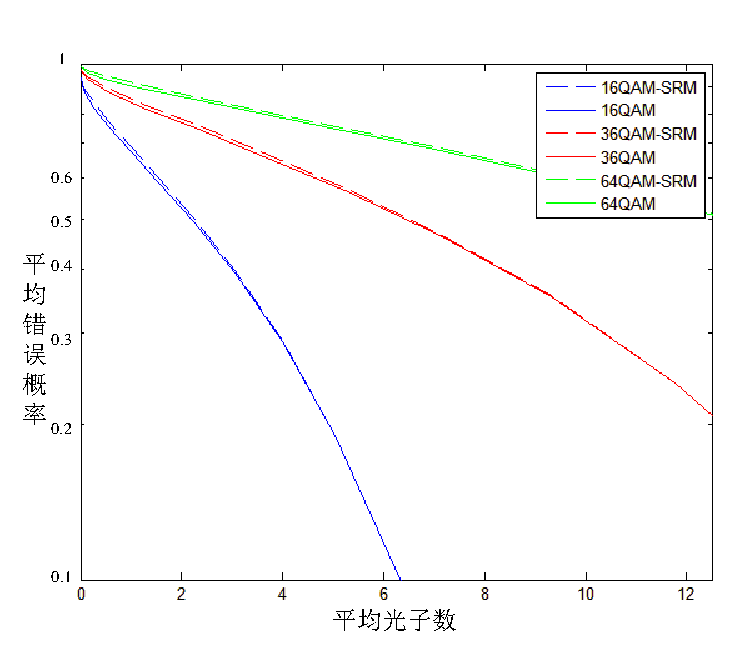
\includegraphics[width=0.6\textwidth]{figures/chap2/QAM-SRM-vs-Helstrom}
  \caption{QAM信号平方根检测与Helstrom极限}
  \label{fig:SRM-vs-Hel}
\end{figure}


\section{现有的量子接收机简介}
自量子检测与估计理论提出以来,如何用现有的物理器件来实现量子接收机,
成为很多研究者关心的问题。二十世纪七十年代,Kennedy和Dolinar等人
首先对二元调制进行探究,分别提出利用线性光学元件实现的Kennedy接收机
和Dolinar接收机\cite{kennedy1973near,dolinar1973optimum}。
后来,经过后续研究者的进一步探索,更多的接收方案
也被提出来了。在本章中,我们回顾一下已被提出的一些重要的接收机
实现方案。
\subsection{二元调制信号量子接收机}
首先,我们来看一些最简单的调制方案——二元调制。
它包括被广泛应用的两种调制方案——OOK和BPSK。
图\ref{fig:signals}显示了他们在星座图上的图像。



这两种调制的最优量子检测性能被Helstrom给出\cite{helstrom1976quantum},
也可以通过平方根检测得到。因为这种两种调制方案是几何均匀对称的,
其对应的幺正矩阵是位移算符$\hat{D}(\alpha)$和$\hat{D}(2\alpha)$,
所以平方根检测性能就是最优量子检测的性能。
我们先求出对应的Gram矩阵
\begin{equation}
\hat{G} = \begin{bmatrix}
            1  &   \xi  \\
            \xi^*  &  1
          \end{bmatrix}
\label{eq:OOK-BPSK-Gram}
\end{equation}
其中$\xi$是两个符号对应的向量的内积,
对于OOK信号,
\begin{equation}
\xi = \bra{0}\ket{\alpha} = e^{-\frac{1}{2}|\alpha|^2},
\end{equation}
而对BPSK信号,
\begin{equation}
\xi = \bra{-\alpha}\ket{\alpha} = e^{-2|\alpha|^2}.
\end{equation}
利用Gram矩阵的表达式\ref{eq:OOK-BPSK-Gram},容易计算出它
的两个特征值为$\lambda_{1,2} = 1 \pm |\xi|$。
根据式\ref{eq:SRM-Pe-GUS},可得平均错误概率为
\begin{equation}
\begin{split}
P_e  &= 1 - \frac{1}{4}(\sqrt{\lambda_1} + \sqrt{\lambda_2})^2\\
     & = \frac{1}{2} \left(1 - \sqrt{1 - |\xi|^2} \right).
\label{eq:OOK-BPSK-Pe-Hel}
\end{split}
\end{equation}

对于BPSK调制集合$\{\ket{-\alpha}, \ket{\alpha} \}$,
在1973年的时候,Kennedy提出\cite{kennedy1973near}利用一个本振场,
对信号进行位移操作$\hat{D}(\alpha)$,
将信号集合变成OOK调制$\{\ket{0}, \ket{2\alpha} \}$,
然后进行直接探测,如图\ref{fig:kennedy-receiver}所示。
如果没有检测到光子(OFF),就判决为信号$\ket{-\alpha}$,
否则(ON)判决为信号$\ket{\alpha}$。
假设$H_0$代表信号$\ket{-\alpha}$,假设$H_1$代表信号$\ket{\alpha}$。
那么,理想条件下,探测的条件概率为
\begin{equation}
\begin{split}
P(\text{OFF}|H_0) & = 1, \\
P(\text{ON}|H_1)  & = 1 - |\bra{0}\ket{2\alpha}|^2 \\
                  & = 1 - e^{-4|\alpha|^2}.
\end{split}
\end{equation}
在通信系统中,先验概率通常是相同的,为$1/2$,那么这种探测的平均错误概率为
\begin{equation}
P_e  = 1 - P(H_0)P(\text{OFF}|H_0) - P(H_1)P(\text{ON}|H_1) = \frac{1}{2}e^{-4|\alpha|^2}.
\label{eq:BPSK-Kennedy}
\end{equation}


\begin{figure}
\centering
  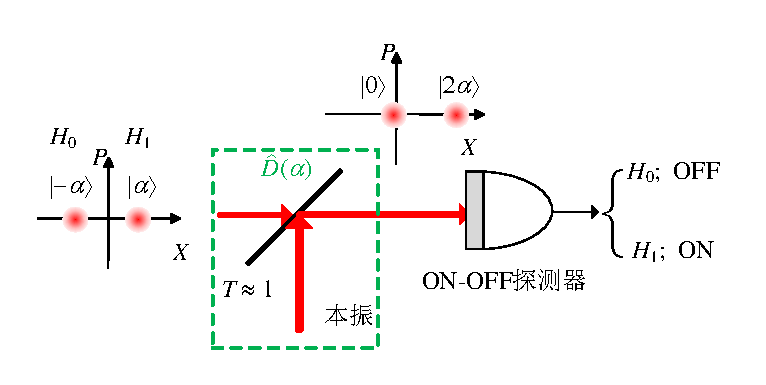
\includegraphics[width=0.8\textwidth]{figures/chap2/Kennedy-receiver}
  \caption{Kennedy接收机示意图}
  \label{fig:kennedy-receiver}
\end{figure}


经典通信系统中,常采用零差接收来探测BPSK信号。
这里假定$\alpha$是实数,根据式\ref{eq:HD-alpha},取$\theta=0$,可知平均错误概率为
\begin{equation}
\begin{split}
P_e & = 1 -\sqrt{\frac{2}{\pi}}\int_0^{\infty} e^{-2(x - \alpha)^2} dx \\
    & = \frac{1}{2}\erfc(\sqrt{2}\alpha).
\end{split}
\end{equation}
对于BPSK信号,经典的零差接收机性能也叫它的标准量子极限(SQL)。
当光子数很大时,利用余误差函数$\erfc$的Chernoff界\cite{chang2011chernoff},
当$x \gg 1$时,$\erfc(x) \approx e^{-x^2}$,
可以得到BPSK零差接收机的渐进性能为
\begin{equation}
P_e = \frac{1}{2}\erfc(\sqrt{2}\alpha) \approx \frac{1}{2} e^{-2\alpha^2}.
\label{eq:BPSK-HD-approx}
\end{equation}
对比式\ref{eq:BPSK-Kennedy}和\ref{eq:BPSK-HD-approx}可以看出,
当光子数较大时,Kennedy接收机的性能比经典的零差接收具有指数倍的增益。
对式\ref{eq:OOK-BPSK-Pe-Hel}做大信号近似,可得在$|\alpha|^2 \gg 1$时,
\begin{equation}
\begin{split}
P_e &= \frac{1}{2} (1 - \sqrt{1 - e^{-4|\alpha|^2}}) \\
    &\approx \frac{1}{4} e^{-4|\alpha|^2}.
\label{eq:BPSK-Hel-approx}
\end{split}
\end{equation}
对比式\ref{eq:BPSK-Kennedy}和\ref{eq:BPSK-Hel-approx}可以看出,
在大信号时,Kennedy接收机与理想的最优量子检测只相差一个常数因子$1/2$,
即Kenendy接收机距最优量子检测只相差3dB。
数值仿真结果如图\ref{fig:Kennedy-error}所示,
可以看到在光子数较小的时候,Kennedy接收机性能没有突破标准量子极限,
只在大信号时能够突破标准量子极限。


\begin{figure}
\centering
  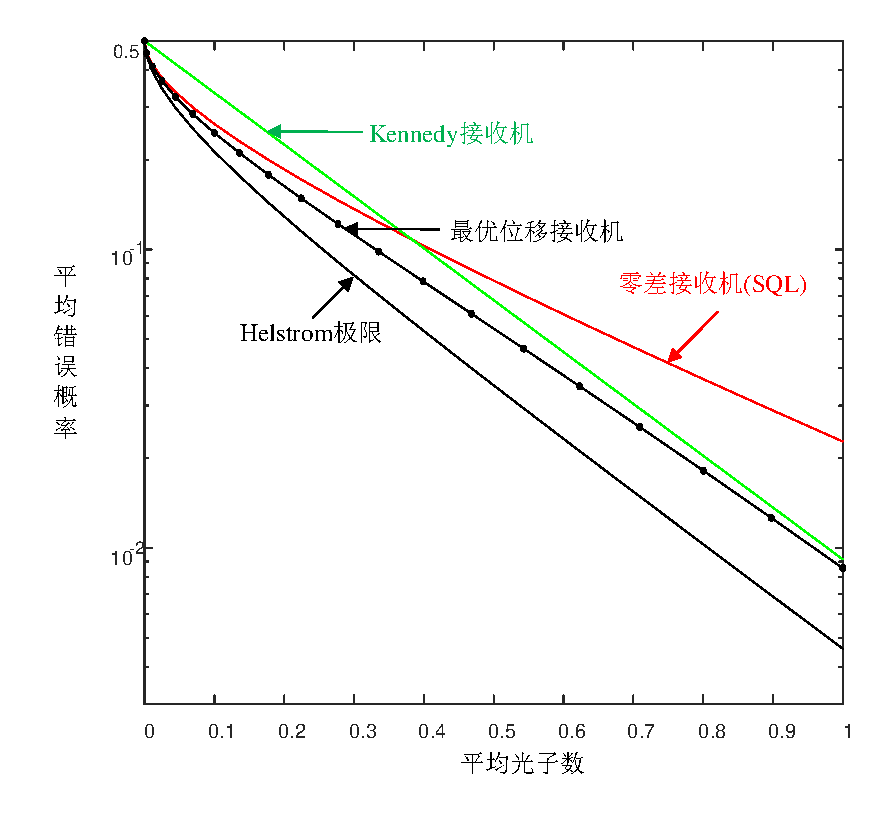
\includegraphics[width=0.6\textwidth]{figures/chap2/Kennedy-error}
  \caption{BPSK信号Kennedy接收机性能曲线}
  \label{fig:Kennedy-error}
\end{figure}


为了解决Kennedy接收机在小信号时的不足,一种采用最优位移
的广义Kennedy接收机(也叫最优位移接收机)被提出\cite{takeoka2008discrimination}。
这种接收机采用与Kennedy接收机相同的结构,但是采用的位移操作
是$\hat{D}(\beta)$,其中位移参数$\beta$通过优化得到。
在这种参数配置下,易得接收机的错误概率为
\begin{equation}
\begin{split}
P_e &= \frac{1}{2} (1 - e^{-|\alpha-\beta|^2} + e^{-|\alpha+\beta|^2}) \\
    &= \frac{1}{2} - e^{-\alpha^2-\beta^2} \sinh(2\alpha\beta).
\label{eq:BPSK-Opt-Kennedy}
\end{split}
\end{equation}
最优位移参数通过求解方程$\partial P_e / \partial \beta  = 0$
得到,即
\begin{equation}
\tanh(2\alpha\beta) = \frac{\alpha}{\beta}.
\end{equation}
从图\ref{fig:Kennedy-error}中可以看到,
最优位移接收机在光子数较小的时候也能突破标准量子极限。
随着光子数增大,最优位移接收机和Kennedy接收机性能越来越接近。
事实上,当光子数很大时,$\tanh(2\alpha\beta) \rightarrow 1$,
最优位移量$\beta \rightarrow  \alpha$。


1973年,Kennedy的学生Dolinar提出Dolinar接收机。
在Kennedy接收机的基础上,Dolinar接收机增加了对本振的实时反馈控制\cite{dolinar1973optimum}。
如图\ref{fig:Dolinar-receiver}所示,位移操作$\hat{D}(\beta)$
的位移量$\beta$在两个策略$u_1(t)$和$u_2(t)$中选择,
每一次单光子探测器接收到一个光子,就切换到另一个位移策略上去。
并且每一个位移策略都是随时间变化的函数。
这里本振的最优控制策略可以通过最优控制理论优化得到\cite{geremia2004distinguishing}。
当本振采用最优控制策略的情况下,可以证明Dolinar接收机
可以达到Helstrom极限,是理论上的最优检测方案\cite{dolinar1973optimum,geremia2004distinguishing}。
2007年,Cook等人从实验上实现了OOK调制的Dolinar接收机\cite{cook2007optical}。

\begin{figure}
\centering
  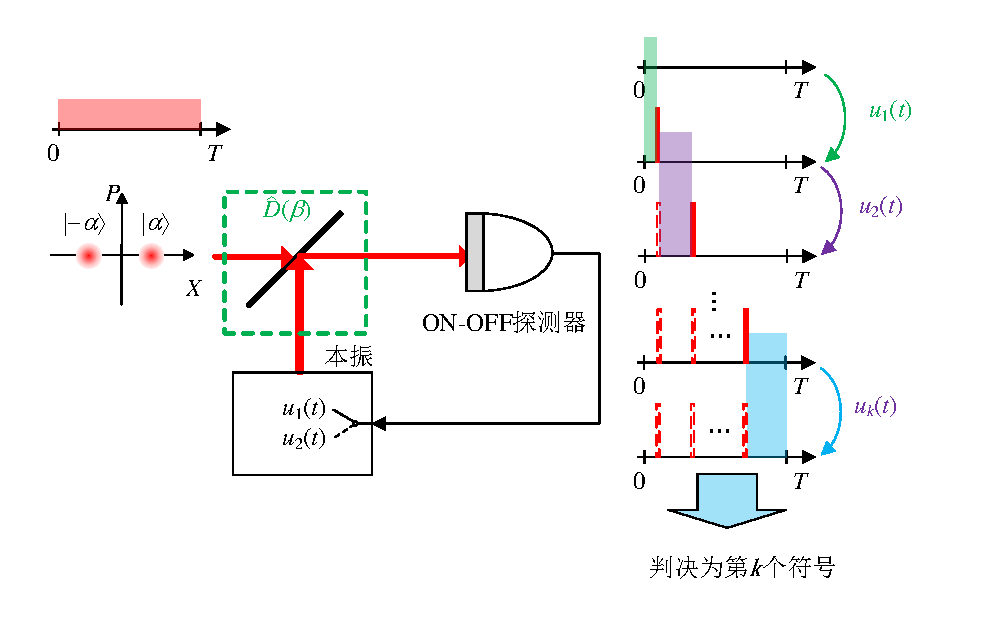
\includegraphics[width=\textwidth]{figures/chap2/Dolinar-receiver}
  \caption{Dolinar接收机原理图}
  \label{fig:Dolinar-receiver}
\end{figure}

Dolinar接收机需要实时反馈控制,这对工程实现要求过高。
一些分区检测方案通过将信号在时间上或者能量上分成
若干份,然后分别采用最优位移接收,弥补了这个不足\cite{vilnrotter2012quantum,li2013optimal,sych2014optimal}。
当分区数目趋近于无穷大时,这种接收机的理论性能和Dolinar接收机一致\cite{sych2014optimal}。

\subsection{多元调制信号量子接收机}
上一小节,我们回顾了最简单的调制信号——二元调制。
这一节我们回顾一下目前研究的比较多的多元调制信号——PSK调制和PPM调制。

QPSK信号用相干态可以表示为
\begin{equation}
\ket{\alpha_i} = \ket{\alpha e^{j \frac{\pi}{2} (i-2)}},i=1,2,3,4.
\end{equation}
我们先来计算一下它的标准量子极限,对于QPSK信号,
外差接收机的性能就是它的标准量子极限。
利用式\ref{eq:Her-receiver-output}或式\ref{eq:Her-receiver-output},
可以得外差接收机平均错误概率为\cite{helstrom1976quantum,kato1999quantum}
\begin{equation}
\begin{split}
P_e &= 1 - \frac{1}{\pi}\int_{Q_1} \exp(-|\beta-\alpha|^2) d^2 \beta \\
    &= 1 - \frac{1}{\pi}\int_0^{\infty} dr \int_{-\pi/4}^{\pi/4} \exp(-\alpha^2 - r^2 + 2\alpha r \cos \theta) r d\theta .
\end{split}
\end{equation}
上式中$Q_1$代表复平面上的区域 $\{\beta|-\pi/4 \le \arg \beta < \pi/4\}$。
%当光子数很大的时候$|\alpha|^2 \gg 1$,利用余误差函数的Chernoff界\cite{chang2011chernoff},
%可得其渐近性能为
%\begin{equation}
%\begin{split}
%P_e &= [2 - \erfc(|\alpha|)]\erfc(|\alpha|) \\
%    &\approx 2e^{-|\alpha|^2}.
%\end{split}
%\end{equation}

因为QPSK具有几何均匀对称性,所以平方根检测就是其最优检测。
QPSK信号对应的Gram矩阵为
\begin{equation}
G = \left[
\begin{array}{cccc}
 1 & e^{-n} & e^{-2 n} & e^{-n} \\
 e^{-n} & 1 & e^{-n} & e^{-2 n} \\
 e^{-2 n} & e^{-n} & 1 & e^{-n} \\
 e^{-n} & e^{-2 n} & e^{-n} & 1 \\
\end{array}
\right].
\end{equation}
这里$n = |\alpha|^2$是信号平均光子数。
根据Gram矩阵可以计算出它的四个特征值为
\begin{equation}
\begin{split}
\lambda_{1,2,3,4} = & e^{-2 n} \left(e^n-1\right)^2,e^{-2 n} \left(e^n+1\right)^2, \\
                    & e^{-2 n} \left(e^{2 n}-1\right),e^{-2 n} \left(e^{2 n}-1\right).
\end{split}
\end{equation}
因此,根据式\ref{eq:SRM-Pe-GUS}可得
\begin{equation}
P_e = 1-\frac{1}{4} \left(\sqrt{1-e^{-2 n}}+1\right)^2.
\label{eq:QPSK-Hel-error}
\end{equation}
在大光子数$n \gg 1$近似条件下,渐近性能为
\begin{equation}
\begin{split}
P_e &= 1-\frac{1}{4} (2 - e^{-2n} + 2\sqrt{1-e^{-2n}}) \\
    &\approx 1-\frac{1}{4} (2 - e^{-2n} + 2- e^{-2n}) \\
    &= \frac{1}{2} e^{-2n} =  \frac{1}{2} e^{-2|\alpha|^2}.
\label{eq:QPSK-Hel-approx}
\end{split}
\end{equation}


\begin{figure}
\centering
  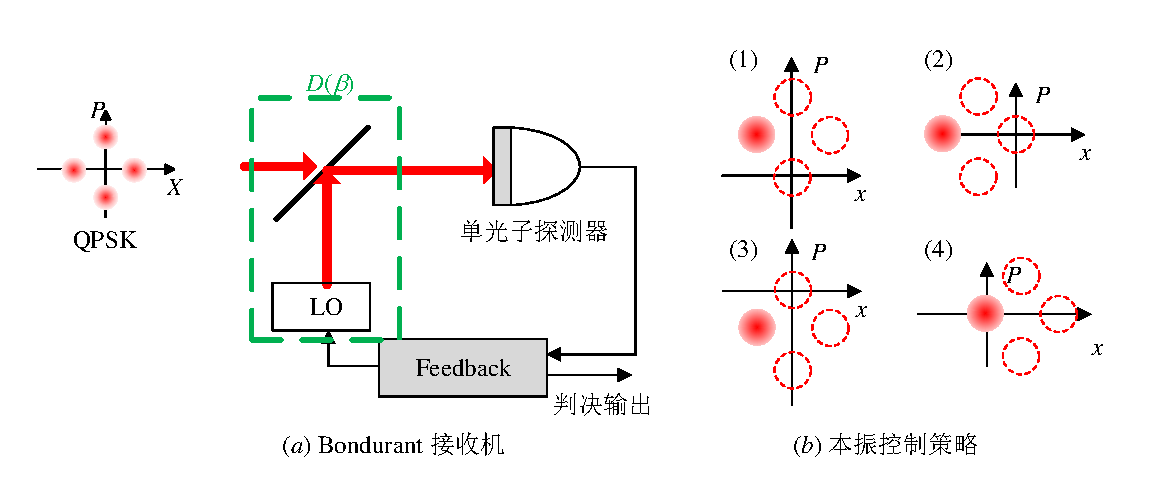
\includegraphics[width=\textwidth]{figures/chap2/QPSK-Bondurant-receiver}
  \caption{QPSK信号Bondurant接收机原理图及反馈控制策略}
  \label{fig:QPSK-Boundurant-receiver}
\end{figure}


1993年,MIT林肯实验室的R. S. Bondurant将Dolinar接收机
的反馈策略推广到QPSK信号,提出两种Bondurant接收机。
这两种接收机只在反馈策略上有所差异,其它都相同\cite{bondurant1993near}。
如图\ref{fig:QPSK-Boundurant-receiver} (\textit{a})所示,
Bondurant接收机由波束分束器、单光子探测器以及一个受反馈控制的本振构成。

第一种Bondurant接收机可以用图\ref{fig:QPSK-Boundurant-receiver} (\textit{b}) 来说明,
在符号开始的时候,接收机选择假设$H_1$,
即假设接收到的符号为$\ket{\alpha_1}$,
反馈策略控制本振将符号1归零,
即控制位移操作$\hat{D}(\beta) = \hat{D}(-\alpha_1)$。
如果在整个符号周期都没有光子计数时间发生,那么选择假设$H_1$输出。
否则,在符号周期中的某个时刻,单光子探测器探测到光子,
那么假设不成立。接着,反馈策略立即控制本振,归零符号2,
即选择假设$H_2$。然后重复上一步,如果继续有光子计数,
则归零符号3,选择假设$H_3$。如果仍然有光子计数,
那么归零符号4,选择假设$H_4$。理想情况下,最多有3个光子计数时间发生。
符号周期结束的时候,选择当前的假设输出。
和Dolinar接收机一样,Bondurant接收机也采用实时反馈控制策略,
但是在每两个光子到达的时间间隔之间,Bondurant接收机的本振是恒定的。

若先验概率相同,第一种Bondurant接收机的平均错误概率为\cite{bondurant1993near}
\begin{equation}
P_e = (\frac{3}{4} + |\alpha|^2) e^{-2|\alpha|^2}.
\end{equation}
当平均光子数较大的时候,渐近性能为
\begin{equation}
P_e \approx |\alpha|^2 e^{-2|\alpha|^2}.
\label{eq:QPSK-Bondurant-approx}
\end{equation}
对比\ref{eq:QPSK-Hel-approx}和\ref{eq:QPSK-Bondurant-approx}
可以看出,第一种Bondurant接收机渐近性能的指数项与最优检测相同。

对于第二种Bondurant接收机,
也是依次归零符号1符号2,但是
在第2个光子到达的时候,反馈控制策略有所不同。
设$t_1$和$t_2$分别代表第1个光子和第2个光子达到的时间。

(a) 如果 $t_1 \le t_2 - t_1$,那么归零符号3,
如果没有光子计数发生了,则选择假设3,否则选择假设4。

(b) 如果 $t_1 > t_2 - t_1$,那么归零符号4,
如果没有光子计数发生了,则选择假设4,否则选择假设3。

在这种策略配置下,接收机的平均错误概率为\cite{bondurant1993near}
\begin{equation}
\begin{split}
P_e  =& \frac{9}{4} e^{-2n} - 2 e^{-3n} + n e^{-3n} \\
      &  + \frac{1}{2} e^{-4n} - n e^{-4n}. 
\end{split}
\end{equation}
上式中$n=|\alpha|^2$为信号平均光子数。
当光子数很大时,略去高阶小量,得到第2中Bondurant接收机渐近性能为
\begin{equation}
P_e \approx \frac{9}{4} e^{-2n} = \frac{9}{4} e^{-2|\alpha|^2}.
\label{eq:QPSK-Bondurant2-approx}
\end{equation}
对比\ref{eq:QPSK-Hel-error}和\ref{eq:QPSK-Bondurant2-approx}两式
可知,第2中Bondurant接收机渐近性能和最优检测只相差一个常数,比第一种
Bondurant接收机前进了一步。

这两种接收机虽然在信号较大的时候可以突破标准量子极限,
但是在小信号的时候,并没有突破标准量子极限。
后来M{\"u}ller借鉴最优位移接收机的思想,
采用不精确归零的方法,改进了小信号时的
性能,使得Bondurant接收机可以在任意光子数都能突破标准量子极限\cite{muller2014qpsk,muller2014m}。

由于Bondurant接收机也需要实时反馈控制,因此不利于工程实现。
后续的研究者 Izumi 通过前馈的方式,将每一个PSK信号分成若干份,
采用Bondurant接收机相似的策略进行前馈\cite{izumi2012displacement}。通过
这种方式减少了反馈带宽的需求,但是同时却增加了
资源的消耗。

后面的研究者Becerra将最大后验概率归零策略加入归零顺序之中,
在每一次前馈的过程中,选择在当前时刻具有最大后验概率的符号,
进行归零\cite{becerra2011m}。这种策略,可以有效地降低
接收机的平均错误概率。2013年,Becerra用反馈的方式
从实验上对这种策略进行了验证\cite{becerra2013experimental}。
并且,考虑到非理想因素如暗计数、模式失配的影响,
将接收端的探测器换成具有光子数分辨能力的探测器,
可以有效的提高接收机的鲁棒性,可以降低暗计数和模式失配带来的
不利影响\cite{izumi2013quantum,li2013suppressing}。
这个结论也在2015年被Becerra通过实验验证\cite{becerra2015photon}。

至此,原则上可以在实验上实现具有鲁棒性的量子接收机,
但是理论上的最优检测如何实现,仍然是一个需要继续研究的问题。

与上述思想不同的是,M{\"u}ller等人提出一种利用
一个零差接收机和一个Kennedy接收机实现QPSK信号接收的
混合接收机\cite{muller2012quadrature}。
这种方案不用反馈控制,简化了QPSK信号接收机的实现。
这种结构也被K. Li推广到16-QAM信号\cite{李科2014}。

在前面我们回顾了PSK信号的量子接收机,
接下来我们回顾一下PPM信号量子接收机研究现状。

首先,我们来计算一下M阶PPM的标准量子极限。
M阶PPM信号有M个时隙,第$i$个符号只有第$i$个时隙
有脉冲,其他时隙都没有脉冲。以4-PPM为例,
4个信号可以用直积态可以表示为
\begin{equation}
\ket{\alpha}\ket{0}\ket{0}\ket{0}, \ket{0}\ket{\alpha}\ket{0}\ket{0},\ket{0}\ket{0}\ket{\alpha}\ket{0}, \ket{0}\ket{0}\ket{0}\ket{\alpha}.
\end{equation}
在经典光通信中采用直接探测对PPM信号进行检测,
如果第$k$个时隙探测到光子,就判决为第$k$个符号;
如果所有的时隙都没探测到光子,那么就随机选择一个符号输出。
因此这种接收策略的平均错误概率为
\begin{equation}
P_e = \frac{M-1}{M} e^{-|\alpha|^2}.
\end{equation}
对于4-PPM信号,平均错误概率为
\begin{equation}
P_e = \frac{3}{4} e^{-|\alpha|^2}.
\end{equation}

接着我们来求M阶PPM信号的Helstrom极限,因为PPM信号
具有几何均匀对称性,所以平方根检测性能就是其
最优量子检测的性能,也就是Helstorm极限。
首先我们计算其Gram矩阵
\begin{equation}
G = \left[
\begin{array}{cccc}
 1 & e^{-n} & e^{-n} & e^{-n} \\
 e^{-n} & 1 & e^{-n} & e^{-n} \\
 e^{-n} & e^{-n} & 1 & e^{-n} \\
 e^{-n} & e^{-n} & e^{-n} & 1 \\
\end{array}
\right]
\end{equation}
其中$n=|\alpha|^2$,
可以看到,Gram矩阵每一行除了对角元为1,其他元素都为$e^{-n}$。
它是一个循环矩阵,其特征值可以通过对第一行元计算$M$点离散傅里叶变换求得\cite{zxd2004matrix},
\begin{equation}
\lambda_1 = 1 + (M-1)e^{-n}, \lambda_{2...M} = 1-e^{-n}.
\end{equation}
所以M阶PPM最优量子检测的平均错误概率为
\begin{equation}
P_e = 1 - \frac{1}{M^2}(\sqrt{1 + (M-1)e^{-n}} + (M-1)\sqrt{1-e^{-n}})^2.
\end{equation}
当光子数很大时,对上式进行近似,保留二阶项$e^{-2n}$,可得其渐近性能为
\begin{equation}
P_e \approx \frac{(M-1)}{4} e^{-2|\alpha|^2}.
\label{eq:PPM-Hel-error}
\end{equation}

早在1982年,Dolinar就提出一种适用于PPM信号的
条件归零(CPN)接收机\cite{dolinar1982near}。
我们接下来以4-PPM信号为例,来简单介绍一下这种接收机。

条件归零接收机所用的器件和结构与图\ref{fig:QPSK-Boundurant-receiver} (\textit{a})
所示的Boundurant接收机一致,不同的是其反馈控制策略。
在PPM信号的每一个时隙中,
条件归零接收机调整它的本振使得位移操作为$\hat{D}(-\alpha)$或者$\hat{D}(0)$。
当位移操作选择$\hat{D}(-\alpha)$时,
接收机在当前时刻归零脉冲,然后进行直接探测。
当位移操作选择$\hat{D}(0)$时,相当于就是直接检测。
以4PPM为例,它的决策策略可以用如图\ref{fig:CPN-Decision-Tree}
所示的决策树表示出来。
条件归零接收机首先归零第一个时隙,
如果没有光子计数,后三个时隙都进行直接探测,
若都没探测到光子,则判决为符号1,
否则若第$k$个时隙出现光子计数,那么判决为符号$k$。
如果第一个时隙探测到光子,那么后三个时隙
当做一个3PPM信号的条件归零接收机。

\begin{figure}
\centering
  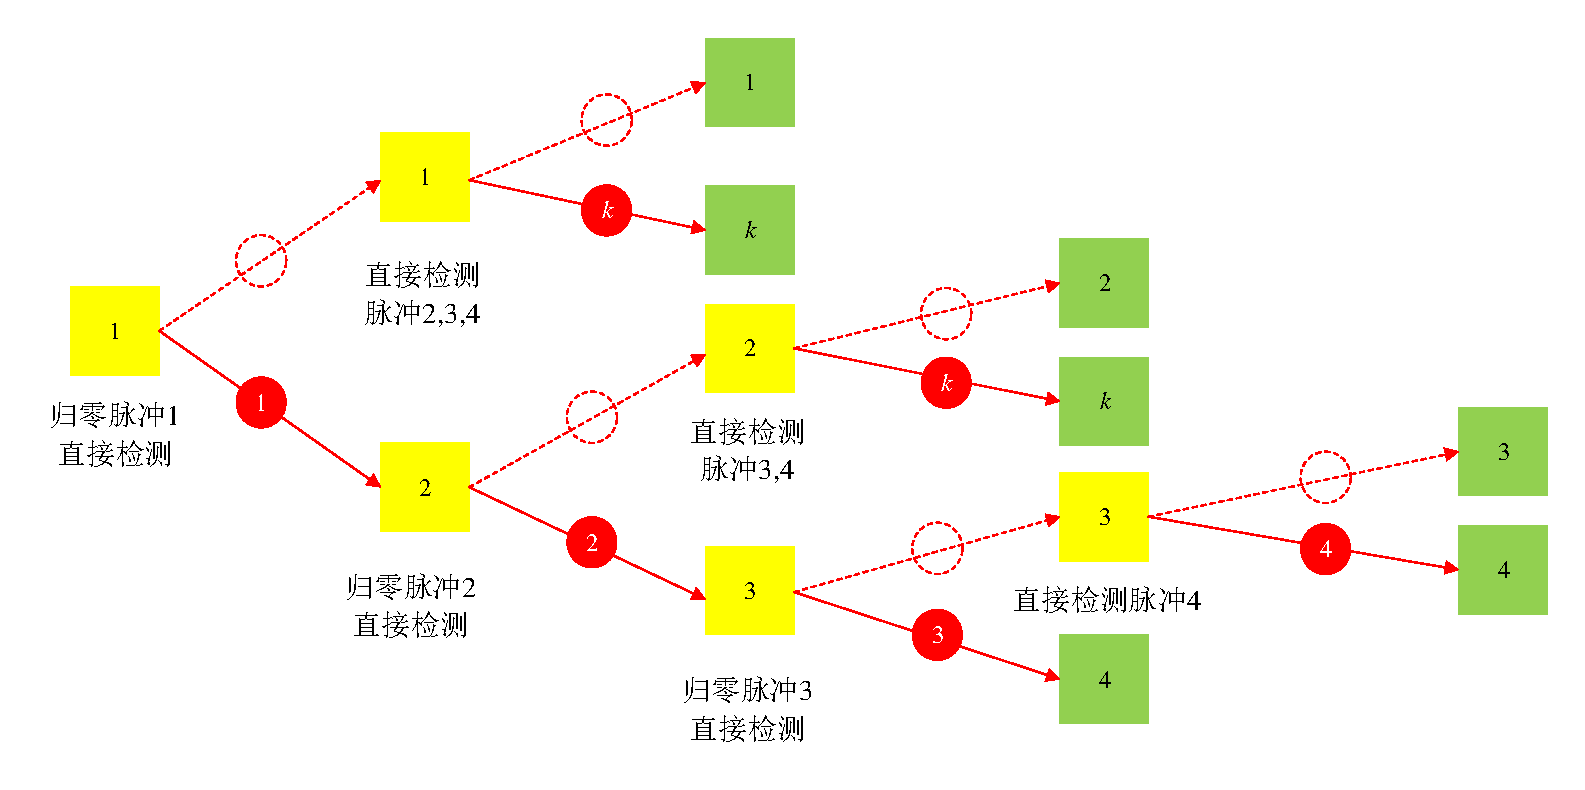
\includegraphics[width=\textwidth]{figures/chap2/CPN-Decision-Tree}
  \caption{4-PPM信号条件归零接收机反馈控制策略决策树}
  \label{fig:CPN-Decision-Tree}
\end{figure}

容易求得,条件归零接收机的平均错误概率为\cite{guha2011approaching,dolinar1982near}
\begin{equation}
P_e = \frac{1}{M}[(1-e^{-|\alpha|^2})^M + M e^{-|\alpha|^2} - 1].
\end{equation}
当光子数很大的时候,其渐近性能为
\begin{equation}
P_e \approx \frac{M-1}{2} e^{-2|\alpha|^2}.
\end{equation}
与式\ref{eq:PPM-Hel-error}对比,可以看到条件归零接收机与最优检测
在大光子数时只相差3dB。

与最优位移接收机思想类似,如果在条件归零接收机每一个时隙里,
采用不精确归零,则可进一步提升接收机在小信号时的性能\cite{guha2011approaching}。
2012年,这两种条件归零接收机被实验验证\cite{chen2012optical}。
Guha等人还提出,可以增加一个相敏放大器(PSA),
从而在位移操作上增加一个压缩操作,可以进一步提升
接收机的性能\cite{guha2011approaching}。
2014年,P. Dalla等人将条件归零接收机的控制策略
进一步改进,在每一个时隙里面采用Dolinar接收机
或者不精确归零接收机,并且每一个时隙的控制参数
都不相同,这些参数通过动态规划算法进行优化,
最终将接收机的性能进一步降低到非常接近Helstrom极限\cite{dalla2014adaptive}。



\subsection{其它类型量子接收机}
在上一小节,我们介绍了目前已经研究得比较多的
几种量子接收机实现方案。
除此之外,还有一些方案也值得借鉴和研究。
2013年,S. Guha等人提出针对任意相干态检测的量子接收机\cite{da2013achieving},
随后该研究组继续提出一种更方便实现的贯序波形归零(SWN)接收机,
用于实现任意相干态接收\cite{nair2014realizable}。
另外,K. Blume等人提出一种基于有限资源量子计算的量子接收机\cite{blume2012ideal},
为研究量子接收机提供新的思路。

与最小错误概率准则不同的是,基于最大无歧义概率准则设计的
无歧义态区分(USD)接收机也被研究人员关注,这种测量方案
理论上不存在错判的概率,但是存在无法判断的概率\cite{becerra2013implementation}。



\section{量子信道编码理论}

在经典信息论中,用Shannon熵来度量一个经典概率分布的不确定度\cite{jd2001xxlybm},
在量子信息论中,描述系统不确定度的是von Neumann熵,定义为\cite{nielsen2005qcqi,nielsen2010quantum}
\begin{equation}
S(\hat{\rho}) = -\Tr\left( \hat{\rho} \log_2 \hat{\rho} \right).
\end{equation}
$\hat{\rho}$是密度矩阵,若$\hat{\rho}$的特征值为$\lambda_x$,
那么上式可以改写为
\begin{equation}
S(\hat{\rho}) = -\sum_x \lambda_x \log_2 \lambda_x.
\end{equation}
这与Shannon熵的形式一致,
为方便记,可以定义$0\log_2 0=0$,便于后续表达。

通过量子信道传递经典信息
需要在发送端将要发送的符号$x \in X$
映射到对应的量子态$\hat{\rho}_x$,然后
将它发送出去,设该信道为$\mathcal{H}$,
每一个量子态对应的先验概率为$p_x$。
这些量子态构成一个混合量子态$\sum_x p_x\hat{\rho}_x$,它的熵满足如下不等式\cite{nielsen2005qcqi}
\begin{equation}
\sum_x p_x S(\hat{\rho}_x) \le S(\sum_x p_x\hat{\rho}_x) \le \sum_x p_x S(\hat{\rho}_x) + H(p_x).
\label{eq:QI-low-up-bound}
\end{equation}
其中$H(p_x)$表示先验分布$p_i$的Shannnon熵。

在接收端,接收机采用一组POVM测量$\hat{\Pi}_y$
进行探测,每一个测量对应的输出为$y \in Y$,
探测的条件概率为
\begin{equation}
P(x|y) = \Tr(\Pi_x \hat{\rho}_y ).
\end{equation}
那么该系统传递的交互信息量为
\begin{equation}
I_1(p_x, \hat{\Pi}_x) = \sum_x p_x \sum_y P(y|x) \log_2  \frac{P(y|x)}{\sum_z p_z P(y|z)}.
\end{equation}
对于给定的符号集合,记交互信息量的最大值为
\begin{equation}
C_1= \sup_{p_x,\hat{\Pi}_y} I_1(p_x, \hat{\Pi}_x).
\end{equation}
它是通过该符号集合对应的单个量子信道$\mathcal{H}$
所能获取的最大信息量。


与上述类似的讨论,我们考虑该单个量子信道的直积信道
$\mathcal{H}^{\otimes n}=\mathcal{H}\otimes\cdots \otimes \mathcal{H}$,
此时输入符号集合为$X^n$,对于其中的每一个符号序列$u = (x_1, x_2, ..., x_n)$,
我们将它映射到直积态
\begin{equation}
\hat{\rho}_u = \hat{\rho}_{x_1}\otimes \hat{\rho}_{x_2}\otimes \cdots \otimes \hat{\rho}_{x_n}.
\end{equation}
设$p_u$是该序列的先验概率,接收端采用POVM测量$\hat{\Pi}_u$进行探测,
我们可以得到交互信息量$I_n(p_u, \hat{\rho}_u)$,
记交互信息量最大值为
\begin{equation}
C_n= \sup_{p_u,\hat{\Pi}_u} I_n(p_u, \hat{\Pi}_u).
\end{equation}
它满足超加性
\begin{equation}
C_n + C_m \le C_{n+m}
\end{equation}
在经典的无记忆信道中,只能取等号,
在量子信道中,可以取不等号,
它存在极限
\begin{equation}
C = \lim_{n \rightarrow \infty} C_n / n
\end{equation}
被称为信道$\mathcal{H}$的信道容量。
经过A. S. Holevo, P. Hausladen,W. K. Wootters等人的努力,
证明了对任意量子态$\{\hat{\rho}_x\}$,信道$\mathcal{H}$的容量为\cite{holevo1973bounds,hausladen1996classical, holevo1996capacity}
\begin{equation}
C = \max_{p_x}\left[ S(\sum_x p_x \hat{\rho}_x) - \sum_x p_x S( \hat{\rho}_x) \right].
\end{equation}
这个容量也称为量子信道$\mathcal{H}$的Holevo容量。
利用式\ref{eq:QI-low-up-bound},可知
\begin{equation}
C \le \max_{p_x}H(p_x).
\end{equation}
当且仅当各量子态之间互相正交时取等号。

如果将量子态放宽到任意量子态,
可以证明,对于能量和带宽受限的条件下,
玻色子场可以最大化信道容量\cite{yuen1993ultimate}。
取符号集合$X = \mathbb{N}$,
$\hat{\rho}_n = \ket{n}\bra{n}$为Fork态,
且先验分布$p_n= N^n(1+N)^{-(n+1)}$,
其中$N$为发送的平均光子数。
此时具有的最大容量
\begin{equation}
C(N) = (N+1)\log_2(N+1) -N \log_2 N.
\label{eq:Boson-capacity}
\end{equation}


量子信道编码定理指出,可以通过对某些特定的长度为$N$的编码码字,
进行联合检测,就有可能随着长度$N$的增大,交互信息量
可以任意逼近Holevo容量\cite{hausladen1996classical, holevo1996capacity}。
因此,两个重要的任务就是找到合适的编码以及
有效的联合检测方案。
1996年,Hausladen采用随机编码和平方根检测的方案
证实对纯态信号集合可以逼近Holevo容量。
近年来,结构化光学接收机\cite{guha2011structured}、
序贯测量方案\cite{giovannetti2012achieving}
以及无歧义态区分方案\cite{takeoka2013achieving}
逼近Holevo容量已被报道。
此外通过极化编码和平方根检测的方案也
被证明可以逼近Holevo容量\cite{guha2012polar}。
但是这些接收机实现都还比较复杂,
不利于工程实现,因此探索方便工程实现的
联合检测接收机是一件十分重要的事情。




\chapter{QAM信号量子接收机}
在上一章中,我们回顾了现有的一些量子接收机实现方案,
包括二元检测和多元的PSK和PPM检测量子接收机。
但是到目前为止,专门针对QAM信号设计的量子接收机
研究还比较少。然而,QAM信号具有很高的频谱效率,
已被应用到大容量光通信系统之中\cite{winzer2012high}。
因此,研究QAM信号量子接收机是一件很有必要的事情。

\section{QAM信号接收机理论极限}
\subsection{标准量子极限}
在经典通信系统中,常用外差接收机检测QAM信号,
这种接收机的性能也叫QAM信号的标准量子极限(SQL)\cite{kato1999quantum}。
设$M$阶QAM信号由$M$个相干态构成,如图\ref{fig:QAM-signals}所示,
显示的是16-QAM和36-QAM星座图。假设$M$阶QAM信号每一个
正交幅度$X$或$P$都可以取$L$个不同的值,那么$M=L^2, L=3,4,5...$。
设这$L$元基本符号集合为$\Omega = \{-(L-1) + 2(i-1) | i=1,2,...,L\}$,
那么$M$阶QAM信号
可以表示为
\begin{equation}
\ket{\alpha_{uv}} = \ket{\alpha(u + j v)}, (u, v) \in \Omega. 
\end{equation}
这里$j=\sqrt{-1}$。例如,16-QAM信号就可以用相干态表示为
\begin{equation}
\begin{split}
\ket{\alpha_{1,1}} &= \ket{\alpha(1 + j )}, \\
\ket{\alpha_{1,3}} &= \ket{\alpha(1 + j 3)}, \\
\ket{\alpha_{1,-1}} &= \ket{\alpha(1 - j )}, \\
                &\vdots                      \\
\ket{\alpha_{-3,-3}} &= \ket{\alpha(-3 - j 3)}.
\end{split}
\end{equation}
这里取$\alpha > 0$,那么M阶QAM信号信号平均光子数为
\begin{equation}
\begin{split}
n &= |\alpha|^2 \frac{1}{M}\sum_{u \in \Omega}\sum_{v \in \Omega} (u^2+v^2)\\
  &= \frac{2}{3}(M-1) |\alpha|^2.
\end{split}
\end{equation}


\begin{figure}
\centering
  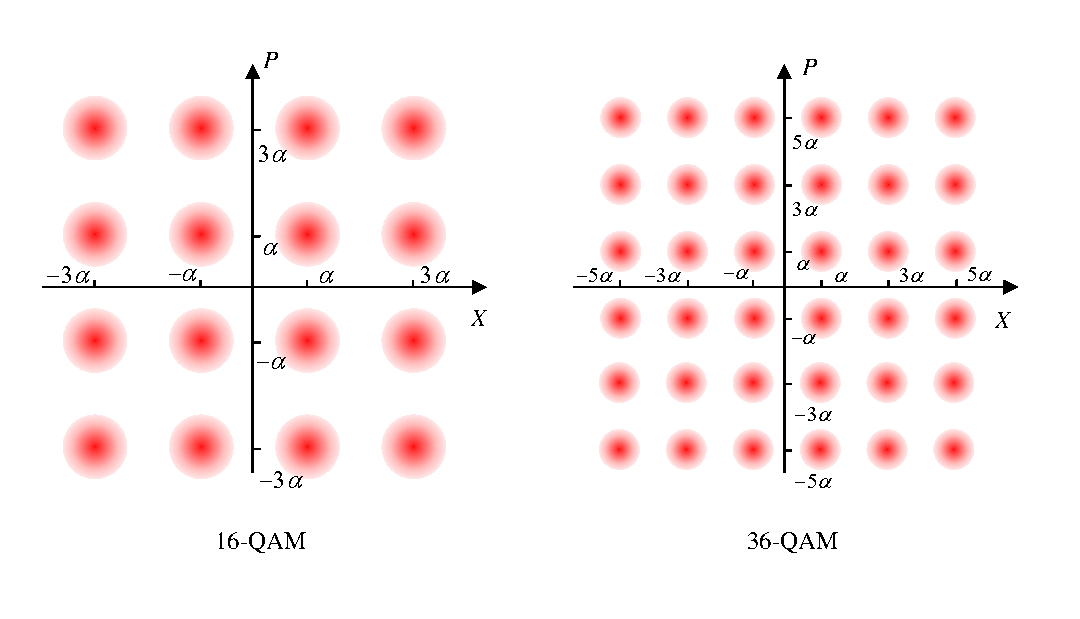
\includegraphics[width=0.8\textwidth]{figures/chap3/QAM-signals}
  \caption{QAM信号星座图}
  \label{fig:QAM-signals}
\end{figure}


下面我们来计算一下QAM信号的标准量子极限。
利用式\ref{eq:Her-receiver-output}可得理想情况下,
外差接收机的概率密度函数为\cite{kato1999quantum}
\begin{equation}
p(x_c, x_s| u, v) = \frac{1}{\pi} \exp[-(x_c - u\alpha)^2 - (x_s - v\alpha)^2]
\end{equation}
这里$x_c$和$x_s$对应于式\ref{eq:Her-receiver-output}中的$\alpha_1$和$\alpha_2$,
是接收机输出的两个正交幅度观测量。
根据贝叶斯检测理论,最优判决区域为
\begin{equation}
D_{u',v'} = \{ (x_c,x_s)| D_L(u') < x_c \le D_U(u'),  D_L(v') < x_s \le D_U(v') \}
\end{equation}
这里$D_U$和$D_L$是两个上下界函数,对给定的参数$L$,
定义为
\begin{equation}
\begin{split}
D_L(u) &= \begin{cases}    
          -\infty     & u < -(L-2)  \\
          \alpha(u-1) & otherwise
         \end{cases}\\
D_U(u) &= \begin{cases} 
          \infty     & u > L-2  \\
          \alpha(u+1) & otherwise
         \end{cases}
\end{split}
\end{equation}
即将复平面划分成如图\ref{fig:QAM-domain-split}所示的$M$个判决
区域,将输出统计量落在某个区域的结果判决为在该区域内的符号。
那么,外差接收机的平均错误概率为
\begin{equation}
\begin{split}
P_e &= 1 - \frac{1}{M} \sum_{u\in\Omega}\sum_{v\in\Omega} \iint_{D_{u,v}} p(x_c,x_s|u,v) dx_c dx_s \\
    &= 1 - \frac{1}{M}[1+(L-1) \erf(\alpha)]^2.
\end{split}
\end{equation}
因此,当平均光子数很大时,即$|\alpha|^2 \gg 1$,
利用余误差函数的Chernoff界\cite{chang2011chernoff},
可得QAM信号外差接收机的渐近性能为
\begin{equation}
\begin{split}
P_e &\approx 2\frac{L-1}{L} e^{-\alpha^2}.
\end{split}
\end{equation}

\begin{figure}
\centering
  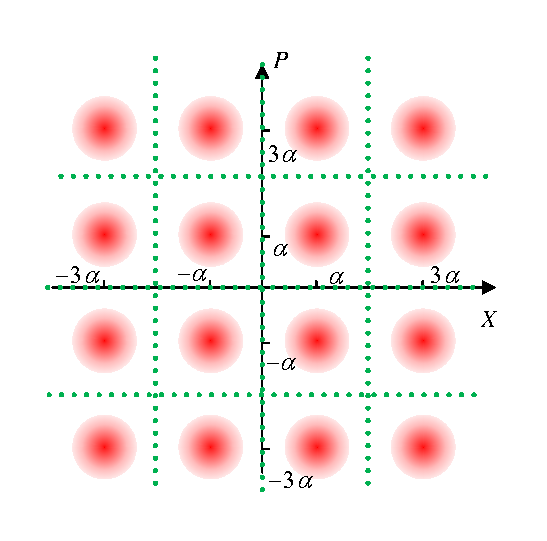
\includegraphics[height=5cm]{figures/chap3/QAM-domain-split}
  \caption{16-QAM信号外差接收判决区域划分示意图}
  \label{fig:QAM-domain-split}
\end{figure}

\subsection{Helstrom极限}


\section{QAM信号Bondurant接收机}


\section{QAM信号自适应分区检测接收机}


\section{QAM信号混合接收机}


\section{三种接收机的对比}


\chapter{二元调制多符号条件归零接收机}
在上一章,我们系统讨论了高阶调制QAM信号的接收方案,
至此,常见的调制方案都已被比较系统的研究。
在这些方案中,通常都是针对单个符号设计的接收方案,
而正如第二章所述,采用针对编码后的多个符号设计的联合检测方案才有可能
逼近Holevo容量。因此这一章我们来讨论最简单的三种
调制方案的一种联合检测方案——条件归零接收机。


\section{MPPM信号条件归零接收机}
首先,我们来考虑一种特殊的编码方案,多脉冲脉冲位置调制(MPPM)信号。
与PPM信号的思想一样,信息被调制在脉冲的位置上面,
具有很高的能量效率,这在深空通信中具有潜在的应用价值\cite{hemmati2006deep}。
与PPM信号不同的是,它的每一个符号通常采用两个或者两个以上的脉冲
来加载信息。采用这种方式,
可以在保证的较高能量效率的同时,
还能有效的克服PPM信号低频谱效率的缺点\cite{sugiyama1989mppm}。
这在深空通信如地月通信、卫星到卫星通信等场景
具有潜在的优势\cite{hemmati2006deep,waseda2011numerical}。

\subsection{MPPM信号标准量子极限}
首先,我们先来从数学上定义MPPM信号符号集合。
设每一个MPPM信号符号有$M$个时隙,对每一个符号,
都有$L$个时隙有脉冲,而其他$M-L$个时隙没有脉冲,
我们称这种MPPM信号为L-M-PPM信号,如图\ref{fig:MPPM-DD}(\textit{a})所示。
一般的,我们只考虑$L \ge 2$的情形,$L=1$时就退化为单脉冲PPM的情形。
容易知道,这样的L-M-PPM信号的符号集合个数为
\begin{equation}
\binom{M}{L} = \frac{M(M-1)\cdots(M-L+1)}{L!}.
\end{equation}
例如当$M=4, L=2$时,2-4-PPM信号有$\binom{4}{2}=6$个,如果用1代表
有脉冲,而用0代表没有脉冲,那么这些信号可以编码为二进制码字
$\bm{c} = (c_1, c_2, \cdots, c_M)$,对2-4-PPM信号这6个码字为
\begin{equation}
\begin{array}{cccc}
1 & 0 & 0 & 1 \\
1 & 0 & 1 & 0 \\
1 & 1 & 0 & 0 \\
0 & 1 & 0 & 1 \\
0 & 1 & 1 & 0 \\
0 & 0 & 1 & 1   
\end{array}
\end{equation}
在将这些码字映射到量子态时,我们用相干态$\ket{0}$和$\ket{\alpha}$
分别代表0和1,用直积态
\begin{equation}
\ket{\gamma_1}\otimes\ket{\gamma_2}\otimes\cdots\otimes\ket{\gamma_M}, \\
\ket{\gamma_i} = \begin{cases}
                    \ket{0}, & c_i=0, \\
                    \ket{\alpha}, & c_i=1
                \end{cases}
\end{equation}
来表示每一个码字对应的信号。

\begin{figure}
\centering
  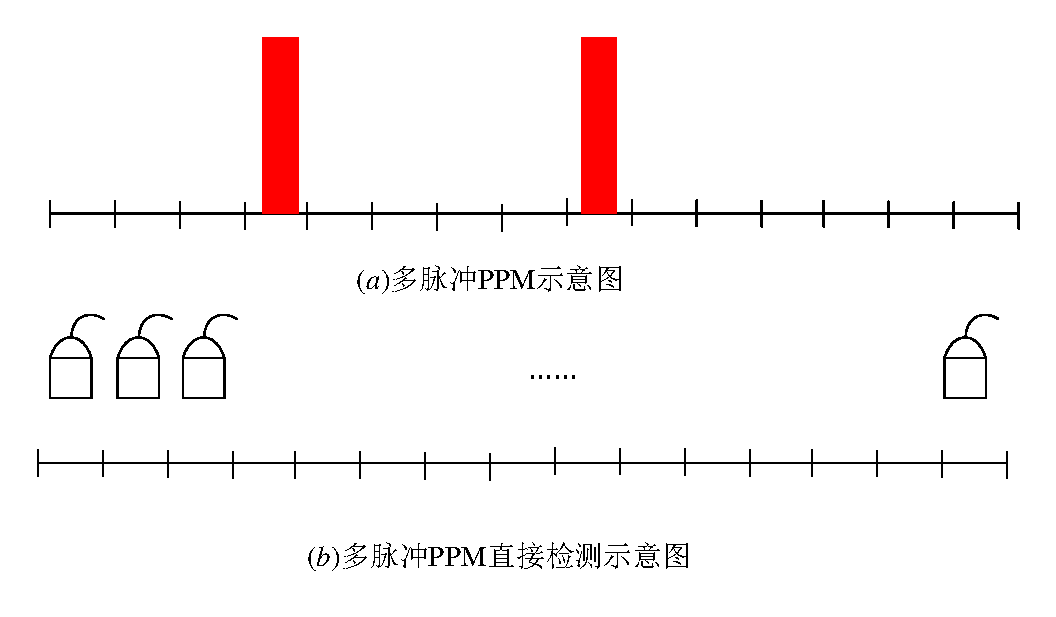
\includegraphics[width=0.8\textwidth]{figures/chap4/MPPM-DD}
  \caption{MPPM信号和直接检测示意图}
  \label{fig:MPPM-DD}
\end{figure}

在经典的光通信系统中,与PPM信号一样,采用直接检测的方法
对MPPM信号进行探测\cite{simon2003multi}。
直接检测探测方法利用一个ON-OFF探测器,
对每一个时隙进行独立的探测。
设每一个时隙的输出为$o_i$,如果有脉冲
$o_i=1$,否则$o_i=0$。
那么$M$个时隙对应的$M$个输出
构成输出序列$\bm{o} = (o_1,o_2,\cdots,o_M)$。
当所有的$M$个时隙都探测完毕,
然后通过最大似然准则进行译码判决\cite{simon2003multi}。
如果所有码字的先验概率是相同的(通信中通常都满足),这种判决准则使得平均错误概率最低。
对于给定的码字$\bm{c}_i$,输出序列为$\bm{o}$的条件概率为
\begin{equation}
\Pr{\bm{o} | \bm{c}_i} = \prod_{k=1}^M \left(1 - e^{-c_{ik}n} \right)^{o_{k}} \left(e^{-c_{ik}n} \right)^{1-o_{k}} .
\end{equation}
其中$\bm{c}_i=(c_{i1},\cdots,c_{iM})$
和$\bm{o}=(o_{1},\cdots,o_{M})$
分别为码字和输出序列,
$n=|\alpha|^2$是一个脉冲的平均光子数。
最大似然准则通过计算对给定的输出序列$\bm{o}$
每一个符号对应的条件概率,
选择出条件概率最大的符号进行判决,
该条件概率也称似然函数。

理想情况下,实际检测到脉冲数目$K \le L$,此时上述
条件概率也即是似然函数变为
\begin{equation}
\Lambda_i = \Pr{\bm{o} | \bm{c}_i} = \begin{cases} 
                                        \left(1 - e^{-n} \right)^{K} \left(e^{-n} \right)^{L-K}, & o_k \le c_{ik} \forall k,\\
                                        0,                                                       & \text{otherwise}.
                                    \end{cases}
\end{equation}
对于给定的码符号集合,$L$是相同的,
所以根据最大似然准则,对给定的输出序列$\bm{o}$,
只要满足$o_k \le c_{ik} \forall k$的码字对应的
似然函数是相同的。此时随机选择一个判决输出。
因此,对给定的码字$\bm{c}_i$,
在探测到$K$个光子时接收机正确探测的概率为
\begin{equation}
\Pr{\bm{c}_i | \bm{c}_i} = \frac{1}{\binom{M-K}{L-K}} \binom{L}{K} \left(1 - e^{-n} \right)^{K} \left(e^{-n} \right)^{L-K}.
\end{equation}
所以,这种检测方案的平均错误概率为
\begin{equation}
\begin{split}
P_e &= \frac{1}{\binom{M}{L}}\sum_{i=1}^{\binom{M}{L}} \sum_{K=0}^{L} \Pr{\bm{c}_i | \bm{c}_i, K}  \\
    &= \sum_{K=0}^{L} \frac{1}{\binom{M-K}{L-K}} \binom{L}{K} \left(1 - e^{-n} \right)^{K} \left(e^{-n} \right)^{L-K}.
\end{split}
\end{equation}
下面我们考虑大信号近似,即当$n \gg 1$时,可以忽略少检测到的脉冲数目大于1个的情况的概率,
即
\begin{equation}
\begin{split}
\Pr{\bm{c}_i | \bm{c}_i} &\approx (1-e^{-n})^L + \frac{L}{M-L+1} (1-e^{-n})^{L-1} e^{-n} \\
                            &\approx 1 - L\left(1 - \frac{1}{M-L+1} \right)e^{-n}.
\end{split}
\end{equation}
因此,这种检测方案的渐近性能为
\begin{equation}
\begin{split}
P_e & \approx L\left(1 - \frac{1}{M-L+1} \right)e^{-n} \\
    & = L\left(1 - \frac{1}{M-L+1} \right)e^{-|\alpha|^2}.
\end{split}
\end{equation}



\subsection{MPPM信号Helstrom极限}
一般而言,MPPM信号并不具有几何均匀对称性,
为了求得这种信号的最优量子检测的性能,
需要如QAM信号那样求解半正定规划问题\ref{eq:Hel-SDP}。
因此,我们需要得到密度矩阵。
与QAM信号不同的是,MPPM信号是直积态,
如果采用QAM信号那种将每一个时隙的信号在Fork态中展开,
然后截取长度为$l$的向量,那么要表达整个直积态信号,
所需要的向量维度为$l^M$,将随着时隙数目$M$指数增长,
这将为计算带来困难。
所以这里我们采用Smit正交化的方法\cite{lzw2010LA,zyh2007szjsff},
构造一组新的基向量$\ket{e_i}$。
为方便计,我们用矢量$\ket{\psi_i}$表示这$N = \binom{M}{L}$个直积态信号,
那么基向量$\ket{e_i}$可以表达为
\begin{equation}
\begin{split}
\ket{u_1} &= \ket{\psi_1}, \ket{e_1} = \frac{\ket{u_1}}{\sqrt{\bra{u_1}\ket{u_1}}}\\
\ket{u_2} &= \ket{\psi_2} - \bra{e_1}\ket{\psi_2}\ket{e_1}, \ket{e_2} = \frac{\ket{u_2}}{\sqrt{\bra{u_2}\ket{u_2}}}\\
          &\qquad\qquad \vdots \\
\ket{u_N} &= \ket{\psi_N} - \sum_{k=1}^{N-1} \bra{e_k}\ket{\psi_N}\ket{e_k}, \ket{e_k} = \frac{\ket{u_N}}{\sqrt{\bra{u_N}\ket{u_N}}}.
\end{split}
\end{equation}
设在该基向量上,$\ket{\psi_i} =\bm{c}_i = (c_{i1} \quad c_{i2} \dots c_{in})^T$,
那么有
\begin{equation}
\begin{split}
c_{11} &= 1, c_{1k}=0 \quad k>1; \\
c_{ii} &= \sqrt{G_{ii} - \sum_{k=1}^{i-1} |c_{ik}|^2 }, c_{ik}=0 \quad k>i, \\
c_{ij} &= \bra{e_j}\ket{\psi_i} \\
       &= \frac{1}{\sqrt{\bra{u_j}\ket{u_j}}} \left( \bra{\psi_j}\ket{\psi_i} - \sum_{k=1}^{j-1} \bra{\psi_j}\ket{e_k} \bra{e_k}\ket{\psi_i} \right)\\
       &= \frac{1}{c_{jj}} \left( G_{ji} - \sum_{k=1}^{j-1} c_{jk}^* c_{ik} \right), \quad j<i.
\end{split}
\end{equation}
这里$G_{ji}=\bra{\psi_j}\ket{\psi_i}$为Gram矩阵元素,
对L-M-PPM信号,
这里两个信号之间的内积为
\begin{equation}
\bra{\psi_j}\ket{\psi_i}=e^{-1/2 d(\bm{c}_i, \bm{c}_j)^2 n}
\end{equation}
这里$d(\bm{c}_i, \bm{c}_j)$这这两个码字的Hamming距离。
利用上述结果,可以得到密度矩阵为
\begin{equation}
\hat{\rho_i} = \ket{\psi_i}\bra{\psi_i} = \bm{c}_i \bm{c}_i^\dagger.
\end{equation}
这里$\bm{c}_i^\dagger$表示$\bm{c}_i$的共轭转置。
一旦将密度矩阵表达为有限维矩阵之后,就可以利用CVX工具箱\cite{cvx,gb08}进行数值求解了。

进一步,利用\ref{eq:Hel-SDP}式,
我们可以求得一个平均错误概率的近似上界。
我们接下来证明一般地,当信号光强很大时$n \gg 1$,
存在非负实数$A_i$使得下式成立
\begin{equation}
\begin{split}
c_{ii} & \ge 1 - A_i e^{-1/2 d_{\min} n}, \\
c_{ij} & \le A_i e^{-1/2 d_{\min} n}, i\neq j.
\end{split}
\end{equation}
其中$d_{\min} = \min_{i \neq j} d(\bm{c}_i , \bm{c}_j)$
是码符号集合的最小汉明距离,容易验证$G_{ij} \le e^{-1/2 d_{\min} n}$。

当$i=1$时,显然成立。
我们假设当$i\le m$时成立,那么当$i=m+1$时,
存在非负实数$A_1, ..., A_{m+1}$,当$n \gg 1$时,有
\begin{equation}
\begin{split}
c_{m+1,j} & \le \frac{G_{j,m+1}}{c_{jj}} \\
       & \le \frac{e^{-1/2 d_{\min} n}}{1 - A_j e^{-1/2 d_{\min} n}}   \\
       & \le e^{-1/2 d_{\min} n} \left(  1 + 2 A_j e^{-1/2 d_{\min} n} \right)  \\
       & \le A_{m+1} A_j e^{-1/2 d_{\min} n}. \\
c_{m+1,m+1} &\ge \sqrt{1 - \sum_{k=1}^{m} A_k e^{-1/2 d_{\min} n} } \\
            &\ge 1 - \frac{1}{2}\sum_{k=1}^{m} A_{m+1} e^{-1/2 d_{\min} n} \\
            &\ge 1 - A_{m+1} A_{m+1} e^{-1/2 d_{\min} n}.
\end{split}
\end{equation}
所以上述命题成立,根据式\ref{eq:Hel-SDP},可得
\begin{equation}
\begin{split}
X_{ii} = \bra{e_i} \hat{X} \ket{e_i} \ge \bra{e_i} \hat{\rho}_i' \ket{e_i} = \frac{1}{N} c_{ii}  .
\end{split}
\end{equation}
所以平均错误概率
\begin{equation}
\begin{split}
P_e &= 1 - \Tr(\hat{X}) =  1 - \sum_i X_{ii} \\
    &\le \frac{1}{N} \sum_i A_i e^{- d_{\min} n}.
\end{split}
\end{equation}
即最优量子检测具有不高于$e^{- d_{\min} n}$形式的渐近性能上界。
事实上,上述结论可以推广到任意量子态集合,
采用最优检测其平均错误概率的渐近性能上界不高于
$e^{-n_{\min}}$,其中$n_{\min} = \min_{ij} |\bra{\psi_i}\ket{\psi_j}|^2$。

利用平方根检测,我们可以得到MPPM大信号时精确渐近性能。
因为
\begin{equation}
\begin{split}
\hat{Z}^2_{ii} \approx \sum_{d=d_{\min}} e^{-1/2 d_{\min} n} = B_i e^{-1/2 d_{\min} n}.
\end{split}
\end{equation}
这里$Z = I -G$,
假定$n \gg 1$,略去高阶小量,其中$B_i$是与码字$\bm{c}_i$距离等于
最小距离码字的个数。
所以由\ref{eq:Gram-approx}式,我们有
\begin{equation}
\begin{split}
P_e &= 1 - \frac{1}{M} \sum_{i=1}^M (1 - \frac{1}{8} \hat{Z}^2_{ii})^2 \\
    &\approx \frac{1}{4M} \sum_{i=1}^M \hat{Z}^2_{ii} \\
    &\approx \frac{1}{4} \sum_i B_i e^{-d_{\min} n} \\
    &\approx \frac{1}{2} D e^{-d_{\min} n}.
\end{split}
\end{equation}
这里$D$是码间距离等于最小距离的码字对数。
例如,对单脉冲PPM信号,任意两个码字间距离都是最小距离2,
所以它的渐近误差性能为$\frac{M(M-1)}{4} e^{-2 n}$.



\subsection{MPPM条件归零接收机}
在第二章,我们简单地介绍了Dolinar在1982年提出的,
针对PPM信号设计的条件归零(CPN)接收机。
我们将该接收机推广到更一般的情况,
用来接收MPPM信号。


\begin{figure}
\centering
  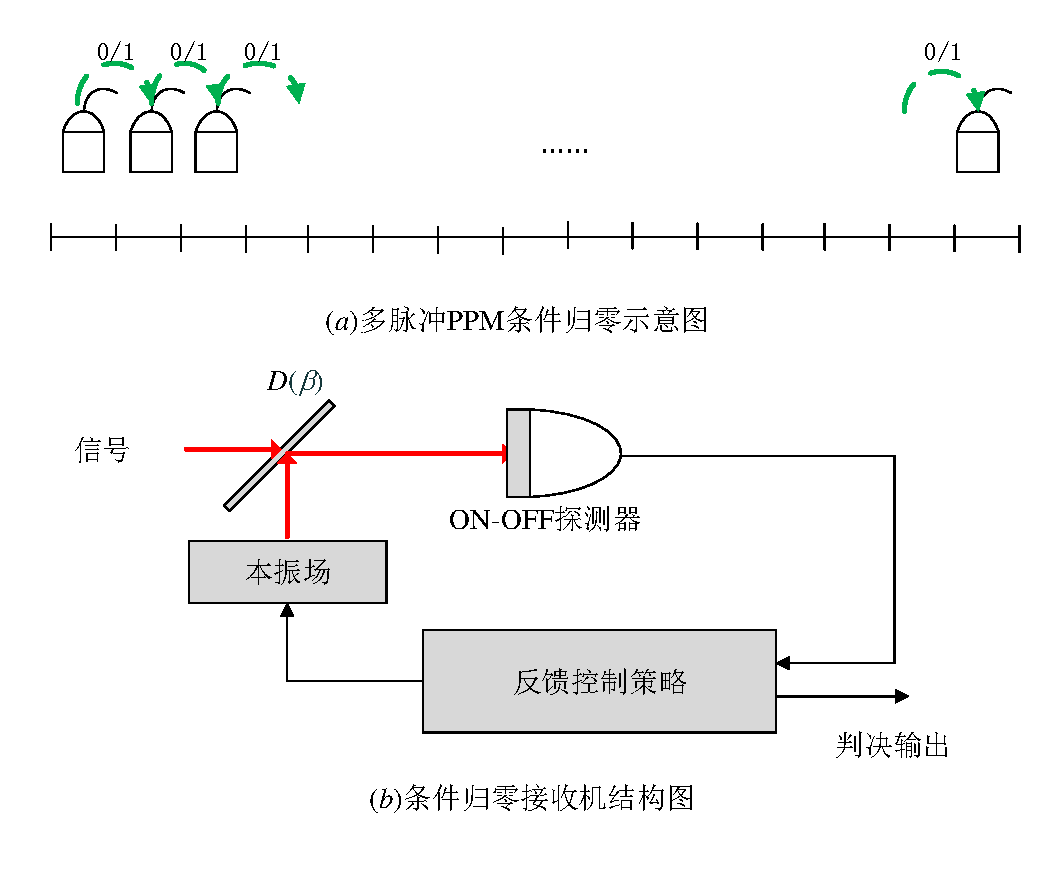
\includegraphics[width=0.8\textwidth]{figures/chap4/CPN}
  \caption{条件归零接收机及接收过程示意图}
  \label{fig:CPN}
\end{figure}

如图\ref{fig:CPN}所示,在每一个时隙,
信号通过一个高透过率分束器
与本振发生干涉,即对信号进行了位移操作,
对MPPM信号而言,位移操作被限定在$\hat{D}(0)$和$\hat{D}(-\alpha)$
中选择一个。
位移后的信号进入单光子探测器或者ON-OFF探测器,
它对应于一个二元POVM测量
\begin{equation}
\hat{\Pi}_0 = \ket{0}\bra{0}, \hat{\Pi}_1 = \hat{I} - \ket{0}\bra{0}.
\label{eq:ONOFF-POVM}
\end{equation}
如果采用$\hat{D}(0)$位移操作,即该时隙采用直接探测,我们记为A类探测,
那么
\begin{equation}
\begin{split}
p_{0|0} &= \Tr[\hat{\Pi}_0 \ket{0}\bra{0}] = 1,\\
p_{1|1} &= \Tr[\hat{\Pi}_1 \ket{\alpha}\bra{\alpha}] = 1-e^{-n}.
\end{split}
\label{eq:CPN-cond-1}
\end{equation}
这里$n=|\alpha|^2$是脉冲的平均光子数,
$p_{0|0}$代表信号在该时隙里没有光脉冲输出为0的条件概率,
$p_{1|1}$代表信号在该时隙里没有光脉冲输出为0的条件概率。
此时单个符号探测的平均错误概率为
\begin{equation}
P_e^{A} = p_1 e^{-n}.
\label{eq:DD-A-error}
\end{equation}
这里$p_1$代表有脉冲的先验概率。
如果采用$\hat{D}(-\alpha)$位移操作,即该时隙归零脉冲后再采用直接探测,我们记为B类探测,
那么
\begin{equation}
\begin{split}
p_{0|0} &= \Tr[\hat{\Pi}_0 \hat{D}(-\alpha)\ket{0}\bra{0}\hat{D}^\dagger(-\alpha)] = e^{-n},\\
p_{1|1} &= \Tr[\hat{\Pi}_1 \hat{D}(-\alpha)\ket{\alpha}\bra{\alpha}\hat{D}^\dagger(-\alpha)] = 0.
\end{split}
\label{eq:CPN-cond-2}
\end{equation}
此时单个符号探测的平均错误概率为
\begin{equation}
P_e^{B} = p_0 e^{-n}.
\label{eq:DD-B-error}
\end{equation}
这里$p_0$代表没有脉冲的先验概率。



反馈策略通过探测器接收到的历史结果和当前结果
来决定下一个时隙采用哪一种位移操作,
即下一个时隙的位移量可以表示为历史的输出和当前的输出的函数。
设当前时刻为$k$,历史输出为$\zeta_{k-1}=(z_1,z_2,...,z_{k-1})$,那么
下一时刻的位移量为
\begin{equation}
\beta_{k+1} = \beta_{k+1}([\zeta_{k-1} , z_k]) = \beta_{k+1}(\zeta_k).
\end{equation}
如果当前时刻的输出为$z_k=0$,即没有光子计数时间发生,
那么下一个时刻的位移量为$\beta([\zeta_{k-1} 0]) = \beta^{z_1...z_{k-1}0}$,
如果$z_k=1$,则$\beta([\zeta_{k-1} 1]) = \beta^{z_1...z_{k-1}1}$,
整个策略可以表示为一颗决策树如图\ref{fig:CPN-strategy}所示。



\begin{figure}
\centering
  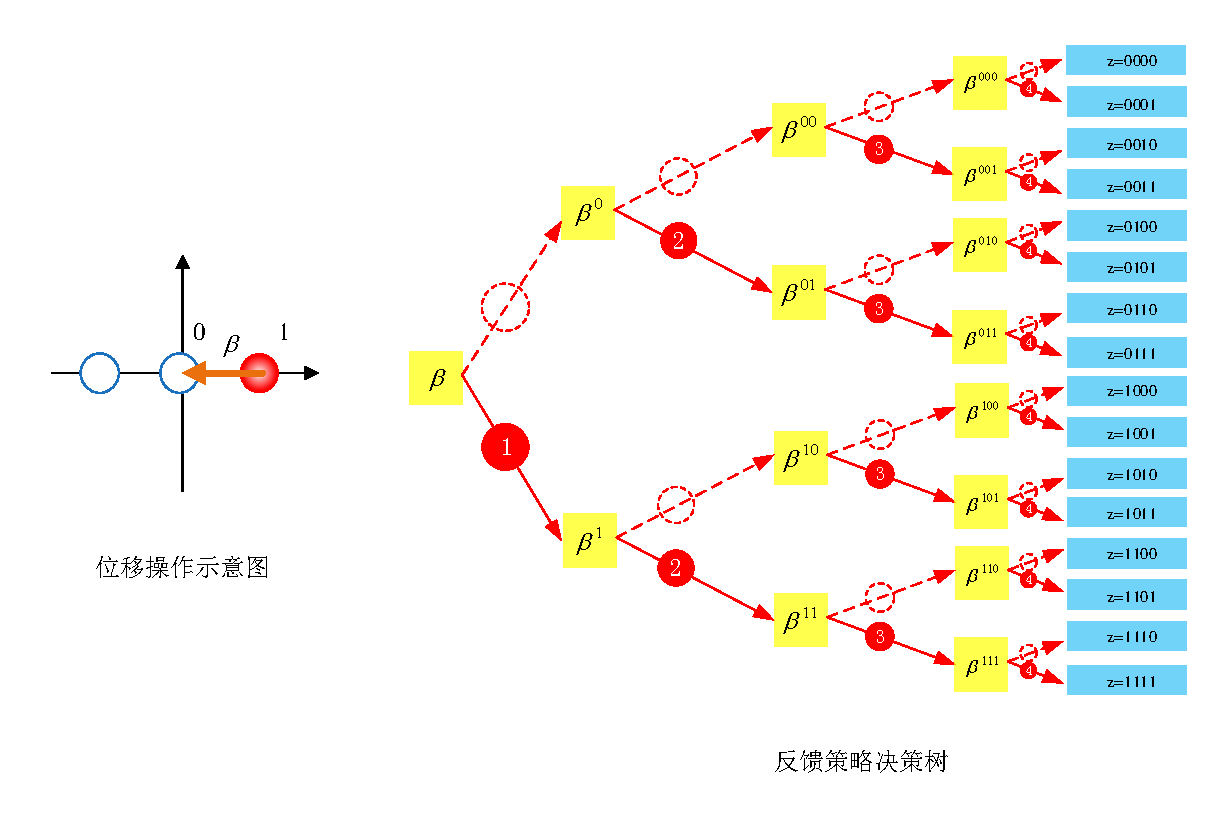
\includegraphics[width=\textwidth]{figures/chap4/CPN-strategy}
  \caption{条件归零接收机反馈策略决策树}
  \label{fig:CPN-strategy}
\end{figure}


当$M$个时隙都探测完毕,设探测器的输出序列为
$\bm{z}=[z_1,z_2,...,z_M]$,我们采用最大后验概率准则(MAP)进行判决,判决函数
\begin{equation}
h(\bm{z}) = \arg\max_i p_{i,\bm{z}}.
\end{equation}
这里$p_{i,\bm{z}}$代表发送第$i$个符号,同时输出序列为$\bm{z}$的联合概率。
那么对所有的符号,平均正确探测的概率为
\begin{equation}
P_c = \sum_z p_{h(\bm{z}),\bm{z}} = \sum_{\bm{z}} \max_i p_{i,\bm{z}}.
\end{equation}
当$M$个符号的先验概率一致时,最大后验概率准则与最大似然准则的结果一致。

现在,我们需要确定函数$\beta_k(\zeta_k)$的形式。
一种简单的取法是$\beta_k \equiv 0$,即每一个时隙都采用直接探测,
此时就是经典的检测方案。
通过观察\ref{eq:DD-A-error}式和\ref{eq:DD-B-error}式
我们可以知道$p_1 < p_0$时,即有脉冲的先验概率
比较大,适合采用B类探测,反之适合采用A类探测。
我们可以取位移策略为最大后验概率策略
\begin{equation}
\begin{split}
\beta_k(\zeta_{k-1}) &= \begin{cases}
                                0, & \text{符号} m_k^*(\zeta_{k-1}) \text{的第} k \text{个时隙没有脉冲}, \\
                                -\alpha, & \text{符号} m_k^*(\zeta_{k-1}) \text{的第} k \text{个时隙有脉冲}.
                             \end{cases} \\
m_k^*(\zeta_{k-1}) &=\arg\max_i p_{i,[z_1,...,z_{k-1}]}.   
\end{split}                          
\end{equation}

一般地,采用最大后验概率策略设计的反馈策略并不一定是最优策略。
为了得到最优策略,我们首先来定义优化目标函数\cite{dalla2014adaptive}
\begin{equation}
\begin{split}
J_k(s_k, \beta_{k+1}) & = \sum_{z' \in \mathcal{Z}_{M-K}} p_{h([\zeta_{k}, z']), [\zeta_{k}, z']}, (k=0,1,...,M-1) \\
J_{M}(s_{M}, \beta_{M+1}) & =  p_{h(\zeta_M), \zeta_M} = p_{h(\bm{z}), \bm{z}}.
\end{split}
\label{eq:reward-to-go-function}
\end{equation}
这里$s_k =s_k(\zeta_{k}) = [p_{1,\zeta_{k}},...,p_{M,\zeta_{k}} ]$是状态向量,
与前面的输出序列有关,
且初始状态$s_0 = [p_1,  ..., p_M] = [1/M, ..., 1/M]$对应于$M$个先验概率。
$\mathcal{Z}_{K} = \{0, 1\}^{\otimes K}$,是$K$维输出序列的状态空间。
容易验证,目标函数具有如下性质
\begin{equation}
J_0 = \sum_{z\in \mathcal{Z}_M} p_{h(z),z} = P_c.
\end{equation}
即$J_0$就是我们最终需要优化的最大平均正确概率。
进一步,我们可以验证$J_k$具有递归关系
\begin{equation}
\begin{split}
J_k(s_k, \beta_k) & = \sum_{z' \in \mathcal{Z}_{M-K}} p_{h([\zeta_{k}, z']), [\zeta_{k}, z']} \\
                  & = \sum_{z' \in \mathcal{Z}_{M-K-1}} p_{h([\zeta_{k}, 0 , z']), [\zeta_{k}, 0 , z']} + \sum_{z' \in \mathcal{Z}_{M-K-1}} p_{h([\zeta_{k}, 1 , z']), [\zeta_{k}, 1 , z']} \\
                  & = J_{k+1}(s_{k+1}([\zeta_{k} 0]), \beta_{k+1}([\zeta_{k} 0])) + J_{k+1}(s_{k+1}([\zeta_{k} 1]), \beta_{k+1}([\zeta_{k} 1])).
\end{split}
\end{equation}
并且状态向量具有如下更新方程
\begin{equation}
\begin{split}
s_{k+1}([\zeta_{k} z_{k+1}]) = s_k \odot [p_{z_{k+1}|1}, p_{{k+1}|2}, \cdots p_{{k+1}|M}]. 
\end{split}
\label{eq:state-transform}
\end{equation}
其中$\odot$是按照元素相乘的哈达马积,$p_{z_{k+1}|i}$表示在发送
码字为第$i$个码字时,第$k+1$个时隙输出为$z_{k+1}$的概率。

为了最大化$P_c$,我们需要优化$J_0$,
原则上我们可以让$\beta_k$取任意复数,
这里我们限定它只能取$\{0, -\alpha\}$中
的一个。根据上述递归关系,我们可以将
该优化问题分解为两个子问题,记$J_k^* = \max_{\beta_{k+1}} J_k(s_k, \beta_{k+1})$,
那么有
\begin{equation}
J_k^*(s_k(\zeta_{k})) = J_{k+1}^*(s_k([\zeta_{k} 0])) + J_{k+1}^*(s_k([\zeta_{k} 0])) 
\end{equation}
因此,可以利用动态规划算法进行优化,
从最后一层进行计算,每一步都对状态空间中的所有
状态进行一次计算,计算完毕后再计算前面一层,直到第0层\cite{dalla2014adaptive}。
但是由于状态空间过大,对$N$个信号,为了得到足够的精度,
需要将状态中每一个元素离散化至少$10^3$个点,
因而每一层需要计算的状态数目为$10^{3N}$个。
由于控制参数被我们限定在两个数范围内取值,
所以对于时隙数目不是很大的情况下,
我们直接进行计算会更加有效。
我们的算法可以归纳如下:

1. 设置初始状态向量 $s_0=[1/M,1/M, ..., 1/M]$。

2. 对每一个$\beta_{1} \in \{0, -\alpha \}$,计算$J_0(s_0, \beta_1)$,
   那么最优正确检测概率和第一个时隙的最优控制策略为
   \begin{equation}
   \begin{split}
   P_c &= \max_{\beta_1 \in \{0, 1 \} } J_0(s_0, \beta_1), \\
   \beta_1^* &= \arg \max_{\beta_1 \in \{0, 1 \} } J_0(s_0, \beta_1).
   \end{split}
   \end{equation}

我们在计算$J_k$的时候,需要计算它的两个子问题。
对给定的$k, s_k, \beta_{k+1}$,
$J_k$可以通过如下算法进行计算:

1. 如果$k=M$,根据\ref{eq:reward-to-go-function}
   式,我们直接返回$s_k$中的最大值作为结果。
   对于其他情况,我们进入步骤2。
   
2. 对当前的状态$s_k$和控制参数$\beta_{k+1}$,
   利用条件概率\ref{eq:CPN-cond-1}式
   和\ref{eq:CPN-cond-2}式,代入状态转移方程\ref{eq:state-transform}
   中计算出新的状态$s_{k+1}([\zeta_k, 0])$
   和$s_{k+1}([\zeta_k, 1])$。
   
3. 然后计算递归两个子问题,对每一个$\beta_{k+2}$,
   分别计算$J_{k+1}([s_{k+1},0], \beta_{k+2})$
   和$J_{k+1}([s_{k+1},1], \beta_{k+2})$,
   设他们的最大值分别为$J_{k+1}^0$和$J_{k+1}^1$,
   那么返回$J_{k+1}^0 + J_{k+1}^1$作为当前函数的计算结果。
   同时可以得到下一个时隙的最优控制策略$\beta_{k+2}^0$
   和 $\beta_{k+2}^1$,分别对应$z_k=0$和$z_k=1$时的
   最优控制参数。
   
   
\begin{figure}
\centering
  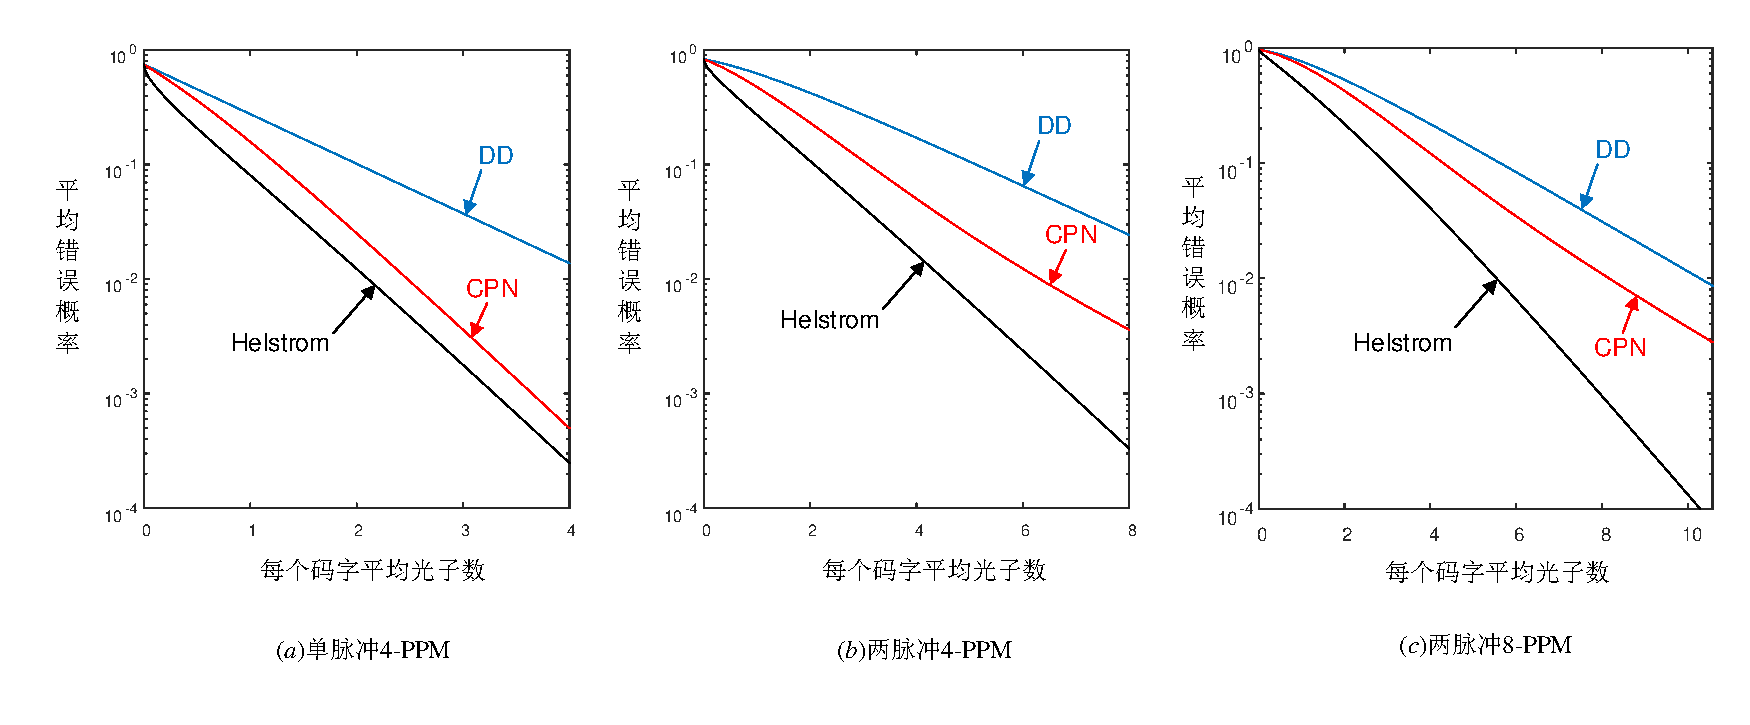
\includegraphics[width=\textwidth]{figures/chap4/4MPPM-error}
  \caption{4个时隙的MPPM性能曲线}
  \label{fig:4MPPM-error}
\end{figure}

\begin{figure}
\centering
  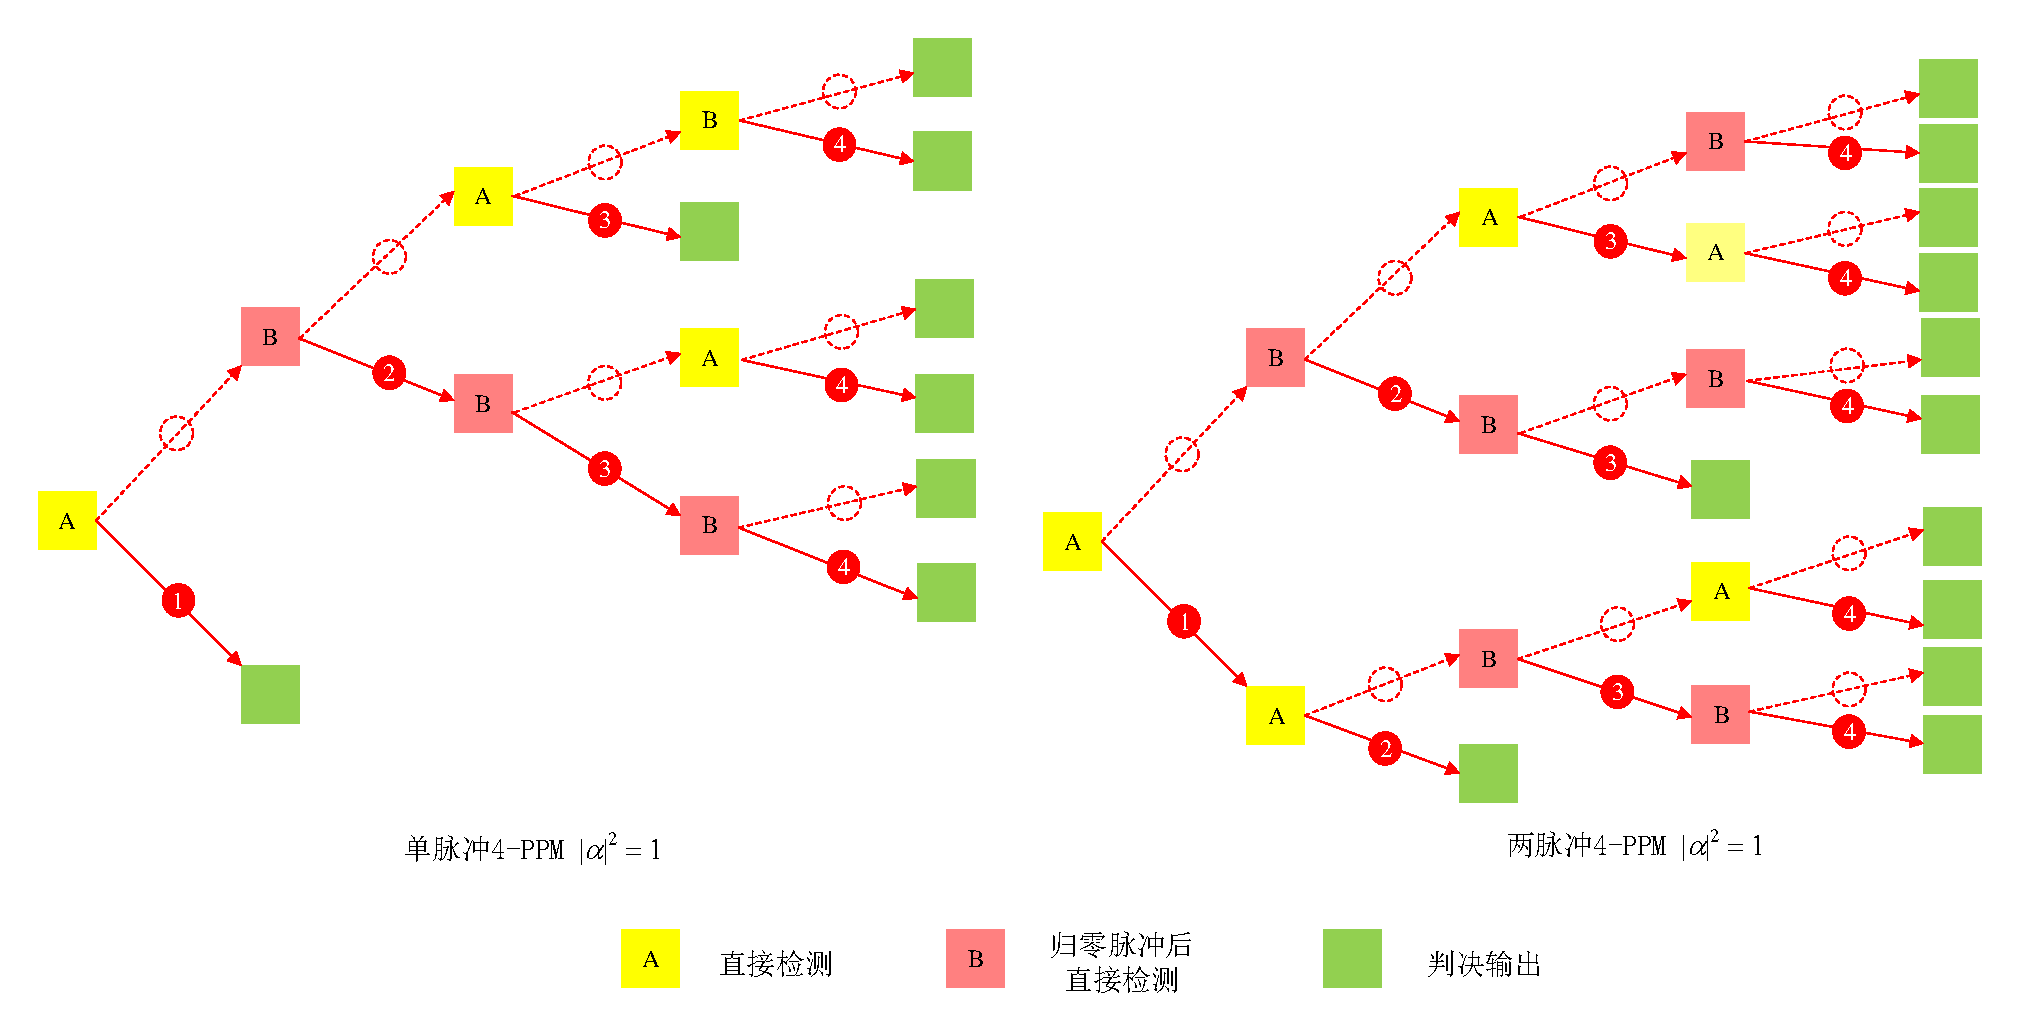
\includegraphics[width=\textwidth]{figures/chap4/2-4-PPM-DT}
  \caption{4个时隙的MPPM控制策略决策树}
  \label{fig:4MPPM-DT}
\end{figure}

利用上述算法,我们分别对4个时隙的单脉冲PPM、
4个时隙两脉冲PPM和8个时隙两脉冲PPM信号进行数值仿真计算,
仿真结果如图\ref{fig:4MPPM-error}所示。
对于单脉冲情况下,就是4-PPM信号,其中蓝色的线代表直接检测(DD)方案,
也就是标准量子极限,红色的线代表条件归零接收机(CPN),
黑色的线代表Helstrom量子极限,
经过对比发现,
虽然通过动态规划优化出来的策略与Dolinar的策略有所差异,
如图\ref{fig:4MPPM-DT}所示,
但是其性能与Dolinar的CPN接收机是相同的,
能够无条件的突破标准量子极限,
即在任意光子数下平均错误概率都比标准量子极限要低。
这表明,最优控制策略并不是唯一的,
而是存在多个最优控制策略。
对于两脉冲情况,从图\ref{fig:4MPPM-error}可以看到,
不论是2-4-PPM还是2-8-PPM信号,
最优控制策略下的条件归零接收机可以
无条件的突破标准量子极限。





\section{编码后二元调制信号条件归零接收机}
在上一小节中,我们讨论了MPPM信号,
它可以看做一种特殊的二进制编码信号,
在这一节里,我们来讨论对任意二进制编码信号,
采用最优控制策略的条件归零接收机,
能否突破传统检测方案的标准量子极限。

\subsection{Hamming码与极化编码}
首先我们来讨论两种重要的编码,
Hamming码和极化编码,以这两种编码为例,分析我们
这种采用最优控制策略的条件归零接收机的性能。

Hamming码是一种古老的编码方式,它是一类参数为
$(2^m-1, 2^m-1-m, m)$的二进制线性码\cite{jd2001xxlybm}。
它的生成矩阵为$G= [ I_k  | A^T]$,
其中$I_k$是$k=2^m-1-m$维单位矩阵,
$A^T$的每一行是是一个长度为$m$的非零二进制向量,
不能为单位向量且两两独立,这种向量一共
有$2^m-1-m$个,按照任意一种排列方式组合成矩阵$A^T$。
它对应的校验矩阵为$H = [A | I_{m}]$满足校验方程
$H G^T = 0$。一般的,我们称这种码字为[$2^m-1$, $2^m-1-m$]Hamming码。
例如[7, 4]Hamming码的生成矩阵为
\begin{equation}
G = \begin{bmatrix}
        1 & 0 & 0 & 0 & 1 & 1 & 0 \\
        0 & 1 & 0 & 0 & 1 & 0 & 1 \\
        0 & 0 & 1 & 0 & 0 & 1 & 1 \\
        0 & 0 & 0 & 1 & 1 & 1 & 1 
    \end{bmatrix}
\end{equation}
利用生成矩阵,我们可以得到所有的码字为
\begin{equation}
c_i = x_i G, i=0,1,...,2^m-1.
\end{equation}
其中$x_i$为数字$i$的$m$位二进制表达。

极化编码是一种利用信道极化特性设计的一种编码方案\cite{arikan2009channel,korada2009polar,wilde2013polar},
采用这种编码方案能够逼近Holevo容量\cite{guha2012polar}。
极化编码也可以看做一种特殊的Reed-Muller(RM)码,
可以通过如下方法生成\cite{arikan2008performance}。
首先生成n阶RM码的生成矩阵
\begin{equation}
G_{RM}(n, n) = F^{\otimes n}.
\end{equation}
其中
\begin{equation}
F = \begin{bmatrix}
        1 & 0 \\
        1 & 1  
    \end{bmatrix}
\end{equation}
$F^{\otimes n}$ 表示n阶张量积。
例如,$G_{RM}(3,3)$为
\begin{equation}
G_{RM}(3,3) = \left[
\begin{array}{cccccccc}
 1 & 0 & 0 & 0 & 0 & 0 & 0 & 0 \\
 1 & 1 & 0 & 0 & 0 & 0 & 0 & 0 \\
 1 & 0 & 1 & 0 & 0 & 0 & 0 & 0 \\
 1 & 1 & 1 & 1 & 0 & 0 & 0 & 0 \\
 1 & 0 & 0 & 0 & 1 & 0 & 0 & 0 \\
 1 & 1 & 0 & 0 & 1 & 1 & 0 & 0 \\
 1 & 0 & 1 & 0 & 1 & 0 & 1 & 0 \\
 1 & 1 & 1 & 1 & 1 & 1 & 1 & 1 \\
\end{array}
\right].
\end{equation}
极化编码只选取满足特定条件的行构成生成矩阵。
首先我们通过如下递归关系
计算极化率向量$z_N = (z_{N,1}, ..., z_{N,N})$
\begin{equation}
\begin{split}
z_{1,1} &= 1/2, \\
z_{2k, j} &= \begin{cases}
                2 z_{k,j} - z_{k,j}^2 & 1 \le j \le k, \\
                z_{k,j-k}^2           & k+1 \le j \le 2k .
            \end{cases}
\end{split}
\end{equation}
接着,我们构造$(1,...,N)$的一个排列$\pi_N = (i_1, ..., i_N)$,
使得在此排列下,极化向量$z_N$是递减的。
那么,对于任意$N=2^n$,$1 \le K \le N$,
[N,K]极化编码矩阵$G_P(N,K)$是由$G_{RM}(n,n)$中
行数在$(i_1,i_2,...,i_K)$中的行构成的子阵。
例如$n=3,K=5$时,极化向量前5个元素对应的下标为
$(8, 4, 6, 7, 2)$,所以
\begin{equation}
G_{P}(8,5) = \left[
\begin{array}{cccccccc}
 1 & 1 & 0 & 0 & 0 & 0 & 0 & 0 \\
 1 & 1 & 1 & 1 & 0 & 0 & 0 & 0 \\
 1 & 1 & 0 & 0 & 1 & 1 & 0 & 0 \\
 1 & 0 & 1 & 0 & 1 & 0 & 1 & 0 \\
 1 & 1 & 1 & 1 & 1 & 1 & 1 & 1 \\
\end{array}
\right].
\end{equation}


\subsection{编码后二元调制信号标准量子极限}
在经典检测方案中,符号探测与译码是两个独立的过程,
因此对编码后的二元调制信号,探测也是通过直接探测每一个时隙进行的,
最后采用最大似然译码准则进行译码。
对于OOK调制,设符号集合为$\{\ket{0}, \ket{\alpha}\}$,这一章$\alpha$都取实数,
在每一个时隙里面,与MPPM一样采用直接探测,可以用式\ref{eq:ONOFF-POVM} 的二元POVM测量表示,
其对应的条件概率由式\ref{eq:CPN-cond-1}给出。
而对BPSK调制,设符号集合为$\{\ket{-\alpha}, \ket{\alpha}\}$,
在每一个时隙里面,采用的是零差接收方式,对应于二元POVM测量
\begin{equation}
\begin{split}
\hat{\Pi}_0 &= \int_{-\infty}^0 \ket{x}\bra{x} dx, \\
\hat{\Pi}_1 &= \int_0^{\infty} \ket{x}\bra{x} dx.
\end{split}
\end{equation}
而条件概率为
\begin{equation}
\begin{split}
p_{0|0} &= \int_{-\infty}^0 |\bra{x}\ket{-\alpha}|^2 dx = \frac{1}{2}(1+\erf{\sqrt{2}\alpha}) \\
p_{1|1} &= \int_0^{\infty} |\bra{x}\ket{\alpha}|^2 dx = \frac{1}{2}(1+\erf{\sqrt{2}\alpha}) 
\end{split}
\end{equation}
这里用0表示符号$\ket{-\alpha}$,而用1表示符号$\ket{\alpha}$,
用$p_{0|0}$和$p_{1|1}$分别表示在符号0和符号1的情况下,探测正确的概率。
在大信号近似下,利用余误差函数的CHernoff界\cite{chang2011chernoff},可得
\begin{equation}
p_{0|0} = p_{1|1} = 1 - \frac{1}{2} e^{-2\alpha^2}.
\end{equation}
因此对应的平均错误概率为
\begin{equation}
p_e \approx \frac{1}{2} e^{-2\alpha^2}.
\end{equation}

对一般的编码信号,
精确地分析误符号率十分困难,
但是可以采用上一章动态规划的方法,
设置控制参数都为0,
就可以得到精确的数值结果。
为了便于进一步分析,这里我们采用近似分析,
只考虑在大信号近似的情况下,即$|\alpha| \gg 1$时,
接收机的误符号率。
我们假设码字的最小汉明距离为$d_{\min}$,
那么在一个码字内,
发生$f = \lceil d_{\min}/2 \rceil$个比特错误
将无法通过译码纠错,
它的概率近似为 $Ae^{-f n}$,其中$A$为某个常数,参数
\begin{equation}
n = \begin{cases}
        |\alpha|^2 & OOK, \\
        2|\alpha|^2 & BPSK.
    \end{cases}
\end{equation}
因为发生更多比特错误的概率是它的高阶小量,可以忽略,
所以经典的探测方案大信号近似下,
平均错误概率$\sim e^{-\lceil d_{\min}/2\rceil n}$,
例如,(7,4)Hamming码的最小汉明距离为3,
所以它的误符号率$\sim e^{-2n}$。
而(8,5)极化码最小汉明距离为2,所以
它的误符号率$\sim e^{-n}$。


\subsection{编码后二元调制信号最优量子检测极限}
根据上一节的分析,我们知道对一个码符号集合,
只要得到符号集合的Gram矩阵,
就可以利用最优量子检测的极限可以通过半正定规划的方法
得到精确。对于任意编码的二元调制信号,Gram矩阵都可以写为
\begin{equation}
G_{i,j} = e^{1/2 d(c_i, c_j) n}.
\end{equation}
其中$c_i$是第$i$个码字,$d(c_i, c_j)$是两个码字的汉明距离,
参数$n$如前面的定义。
根据Gram矩阵,就可以利用CVX工具箱\cite{cvx,gb08}求解问题\ref{eq:Hel-SDP}
得到最优解了。

为了方便分析,我们也采用大信号近似,根据前面的结论,
大信号时的平均错误概率$\sim e^{-d_{\min} n}$,
这里$d_{\min}$为码字的最小汉明距离。





\subsection{编码后二元调制信号条件归零接收机}
对于编码后的二元调制信号,包括OOK调制和BPSK调制,
我们采用与MPPM相似的接收机结构,
只是接收策略不同。

与MPPM信号类似,编码后的OOK信号在每一个时隙里面的
测量策略是一样的,都是从直接检测和归零脉冲后再直接检测
这两种测量方案中,根据历史输出和优化策略选择一种进行探测。
而对于BPSK调制,则有所不同。
在每一个时隙里面,编码后的BPSK调制条件归零接收机在
两种Kennedy接收机中选择一个进行探测。


\begin{figure}
\centering
  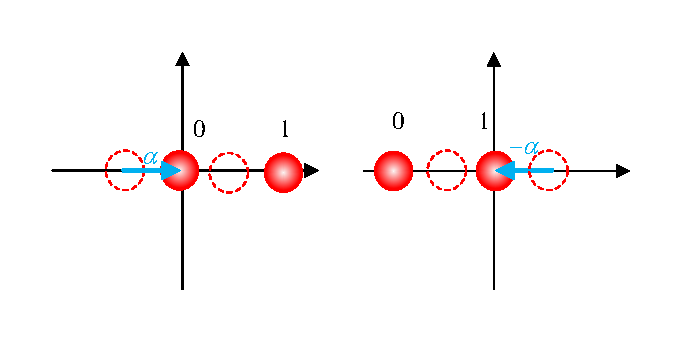
\includegraphics[height=5cm]{figures/chap4/BSPK-AB-receiver}
  \caption{在每个时隙中BPSK调制采用的两种Kennedy接收方案}
  \label{fig:BSPK-AB-receiver}
\end{figure}





如图\ref{fig:BSPK-AB-receiver}所示,
第一种Kennedy接收机通过一个位移操作$\hat{D}(\alpha)$,
将BPSK符号集合变成OOK调制$\{\ket{0}, \ket{2\alpha}\}$
然后直接探测,它对应于二元POVM测量
\begin{equation}
\begin{split}
\Pi_0 &= \hat{D}(\alpha)^\dagger \ket{0}\bra{0} \hat{D}(\alpha) ,\\
\Pi_1 &= \hat{D}(\alpha)^\dagger (\hat{I} - \ket{0}\bra{0}) \hat{D}(\alpha) .
\end{split}
\end{equation}
在这组POVM测量下,探测的条件概率为
\begin{equation}
\begin{split}
p_{0|0} &= 1, \\
p_{1|1} &= 1 - e^{-4|\alpha|^2}.
\end{split}
\end{equation}
这里我们用$p_{0|0}$表示在信号0的情况下,
输出为0,即没有光子计数发生,
而$p_{1|1}$表示在信号1的情况下,
输出为1,即发生了光子计数事件。
第二种Kennedy接收机通过一个位移操作$\hat{D}(-\alpha)$,
将BPSK符号集合变成$\{ \ket{-2\alpha}, \ket{0}\}$
然后直接探测,它对应于二元POVM测量
\begin{equation}
\begin{split}
\Pi_0 &= \hat{D}(-\alpha)^\dagger \ket{0}\bra{0} \hat{D}(-\alpha) ,\\
\Pi_1 &= \hat{D}(-\alpha)^\dagger (\hat{I} - \ket{0}\bra{0}) \hat{D}(-\alpha) .
\end{split}
\end{equation}
在这组POVM测量下,探测的条件概率为
\begin{equation}
\begin{split}
p_{0|0} &= e^{-4|\alpha|^2}, \\
p_{1|1} &= 0.
\end{split}
\end{equation}

\begin{figure}[H]
\centering
  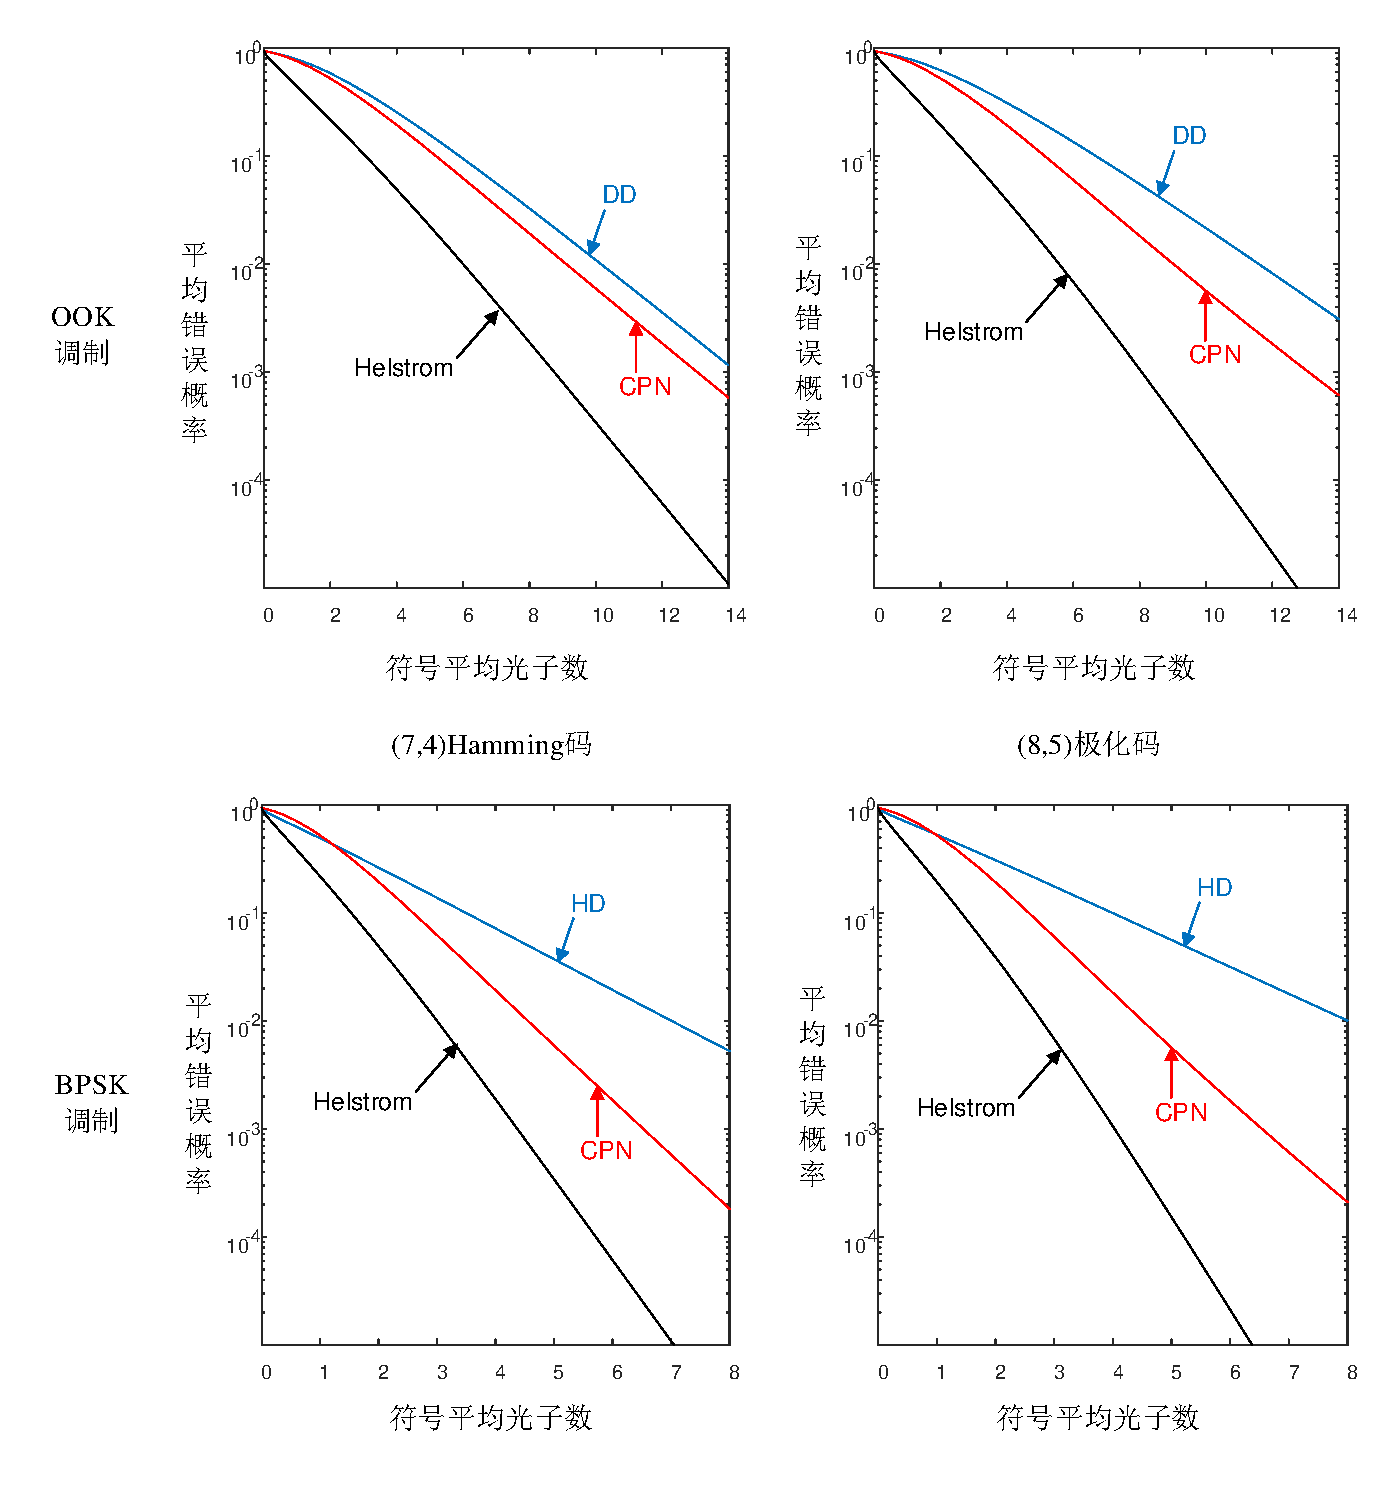
\includegraphics[width=\textwidth]{figures/chap4/OOK-Code-error}
  \caption{OOK信号汉明码和极化码的条件归零接收机性能}
  \label{fig:OOK-Code-error}
\end{figure}


利用上述结果,我们就可以利用式\ref{eq:state-transform}更新状态方程了,
进而采用动态规划的方法对控制策略进行优化。
我们选择了(7,4)汉明码和(8,4)极化码进行数值仿真,
仿真结果如图\ref{fig:OOK-Code-error}所示。
可以看到,对于OOK调制这两种不同的编码方案,
条件归零接收机可以在任意光子数下突破经典检测的极限。
当每个符号的平均光子数为14时,因为每一个Hamming码
码字平均有3.5个脉冲,因此每个脉冲的平均光子数为4,
此时采用条件归零接收机可以有近3dB的收益。
对于极化码,当每个符号的平均光子数为14时,
因为每一个极化码
码字平均有4个脉冲,因此每个脉冲的平均光子数为3.5,
此时采用条件归零接收机有7.4dB的收益。
对于BPSK调制这两种不同的编码方案,
可以看到条件归零接收机在信号较大时才能突破经典检测的极限,
而在码字信号平均光子数小于1时,
这种接收方案反而会比零差接收机要差。
但是当光子数增大时,这种接收方案比经典接收方案的收益
随着显著增大。
对比OOK和BPSK两种调制,可以发现要达到相同的误码率,
在相同的编码情况下,采用BPSK调制的条件归零接收机所需要的
能量更低,因而具有更高的能量效率。


\chapter{量子接收机初步实验研究}
前面两章,我们分别研究了单符号的QAM信号量子接收机,
以及多个符号的编码后二元调制信号量子接收机。
通过理论分析和数值仿真分析,我们证明了
我们提出的量子接收机能够突破经典检测极限——标准量子极限。
然而到目前为止,
从实验上对量子接收机进行论证的工作仅停留在有限的几种方案当中,
对于更多的方案以及他们的工程实现还有待进一步研究。
为了后续的实验研究工作,我们在现阶段进行量子接收机实验平台
搭建工作,希望能够完成初步的实验研究。


\section{实验原理及实验平台搭建}
最早对量子接收机进行实验验证的工作要追溯到2006 年 C. W. Lau等人
开始进行二元调制信号的Kennedy接收机实验和Dolinar接收机的实验验证\cite{lau2006binary},
但是很遗憾受限于实验条件,C. W. Lau 等人设计的Dolinar接收机实验没能突破标准量子极限。
当时实验装置采用空间光路,位移操作通过一个空间光马赫曾德干涉仪实现,
由于对幅度调制的精确控制达不到要求,使得Dolinar接收机性能不理想。
到2007年,R. L. Cook终于从实验上验证了Dolinar接收机能够达到Helstrom极限\cite{cook2007optical}。
从这两个实验及后续的一些实验来看\cite{wittmann2008demonstration,wittmann2010demonstration,tsujino2010sub,
tsujino2011quantum,becerra2011m,chen2012optical,muller2012quadrature,becerra2013experimental,
becerra2015photon},
实验上目前实现量子接收机的难点在于
具有光子数分辨能力的高量子效率低暗计数的单光子探测器和对位移操作的精确实现。
对于前者,实验上通过采用死区时间小并且探测效率在65\%左右的APD单光子探测器实现,
也有实验采用超导TES单光子探测器以达到非常高的量子效率\cite{tsujino2011quantum}。
而具有光子数分辨能力的探测器能够使得接收机鲁棒性更强已被
理论和实验验证\cite{izumi2013quantum,li2013suppressing,becerra2015photon}。
这里我们考虑超导探测器需要很低的温度控制,
对实验环境要求太高,所以我们采用大多数研究组都采用的APD单光子探测器。
我们采购的是EXCELITAS 公司型号为SPCM-AQRH-16单光子探测器,
典型的死区时间为20ns,暗计数只有25cps,在633nm波段探测效率
>65\%。
对于位移操作,实验上有两种实现方案,一种是利用一个马赫曾德干涉仪,它
通过主动的反馈控制将两个臂的光程差进行锁定,
以保证足够的位移操作精度\cite{becerra2013experimental,
becerra2015photon};另一种方案是利用偏振复用方式,
其中一个偏振当做信号而另一个偏振分量当做本振,最后通过一个偏振器(PBS)进行干涉\cite{wittmann2008demonstration,wittmann2010demonstration}。
因为在这种方案中,本振和信号通过相同的光路,所以不存在干涉的两个臂的光程差不稳定的问题,
但是这种方案对信道保偏性和调制器的偏振特性要求较高,只适合空间光路。
由于后面一种方案便于在空间光路中实现,
所以我们采用后面这种方案实现精密的位移操作。


\begin{figure}
\centering
  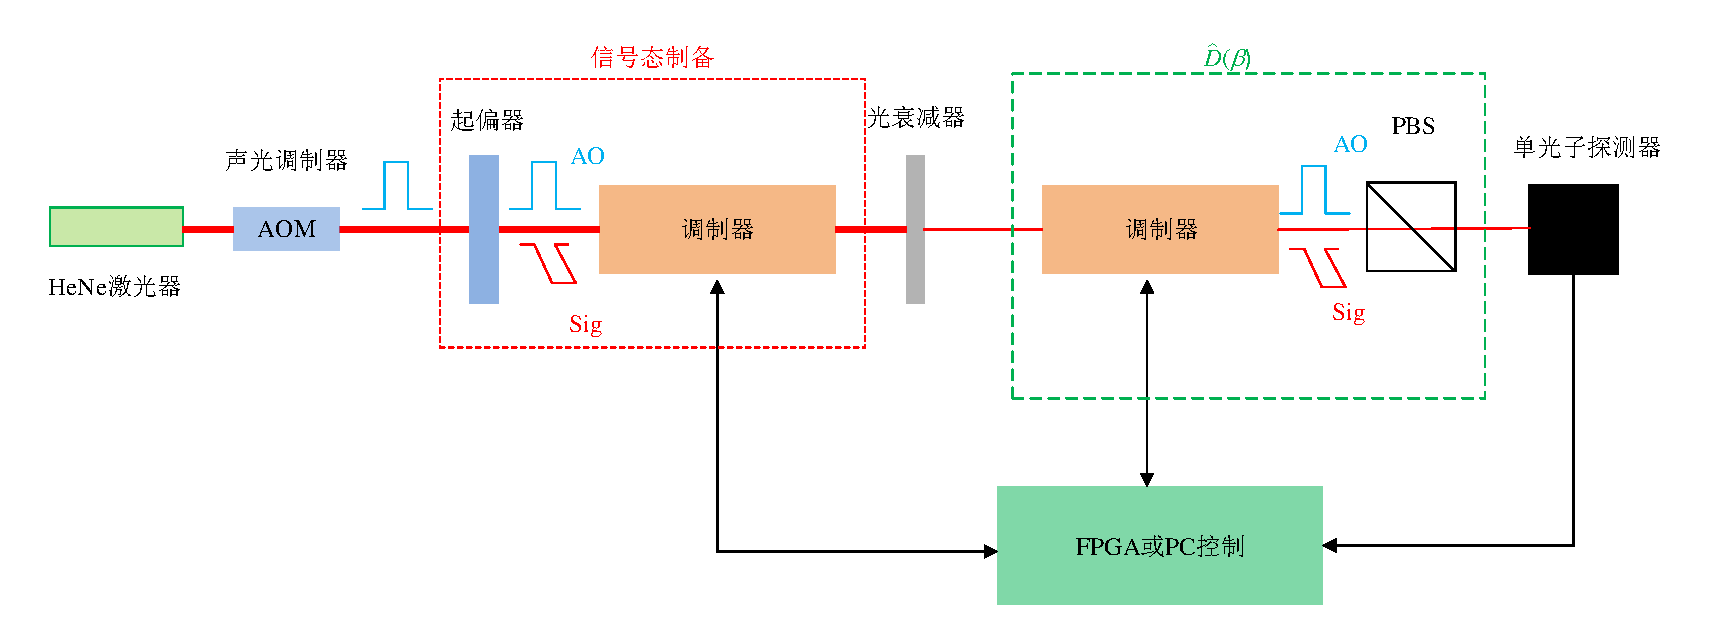
\includegraphics[width=\textwidth]{figures/chap5/experiment-schematic}
  \caption{量子接收机实验原理图}
  \label{fig:experiment-schematic}
\end{figure}



实验原理图如图\ref{fig:experiment-schematic}所示,
HeNe激光器发出的连续光经过声光调制器(AOM)被斩成光脉冲,
然后经过45°放置的起偏器得到强度相等的水平偏振分量和垂直偏振分量。
其中水平偏振分量作为信号态(Sig),垂直偏振分量作为辅助场(AO),在接收端被用作本振场(LO)。
接着,调制器通过基于非线性晶体的电光调制器,
对两个偏振分量进行相移,由于非线性特性导致相移量存在一个差值$\Delta \phi$。
对于BPSK调制,通过控制调制电压使得$\Delta \phi$取$0$和$\pi$,
对于一般的PSK调制只需要控制调制电压就行。
最后信号通过光衰减器模拟的有损空间信道,
到达接收端,这样就完成了信号态的制备。
用琼斯矩阵表示为
\begin{equation}
\ket{\psi_{Sig, AO}}(\Delta \phi) = \begin{bmatrix}
                            e^{j \Delta \phi}\sqrt{n_{Sig}} \\
                            \sqrt{n_{AO}} 
                        \end{bmatrix}
\end{equation}
在接收端接收机通过一个电光调制器
和一个偏振器
实现位移操作,然后进行光子计数。
设调制器导致的相移为$\Delta \phi' + \pi$,
PBS的极化矢量为$\vec{p} = [\sqrt{T} \quad \sqrt{1-T}]$,$T$为透过率,
那么进入单光子计数器钱的光场为
\begin{equation}
\bra{\vec{p}} \ket{\psi_{Sig, AO}}(\Delta \phi + \Delta \phi') \\
             =  \sqrt{T}\sqrt{n_{Sig}} - \sqrt{1-T}\sqrt{n_{AO}} e^{j(\Delta \phi + \Delta \phi')} 
\end{equation}
若PSB与信号偏振态的夹角$\theta$非常小,
那么透过率$T = \cos^2 \theta \approx 1$,
那么上述相当于完成位移操作
\begin{equation}
\hat{D}(\beta) = \hat{D}(\sqrt{n_{AO}}\sqrt{1-T} e^{j \Delta\phi'}).
\end{equation}
特别的,当$T = \frac{n_{AO}}{n_{Sig} + n_{AO}}$时,
到达探测的脉冲中的平均光子数为
\begin{equation}
\bar{n} = \frac{n_{Sig} n_{AO}}{n_{Sig} + n_{AO}} \left|1 - e^{j\Delta \phi + j \Delta \phi'} \right|^2.
\end{equation}
当且仅当$\Delta \phi + \Delta \phi'$ 是$2\pi$的整数倍时,
恰好光强为0,此时位移操作恰好把信号场归零。

\section{Kennedy接收机实验验证}

作为初步实验研究工作,我们对最简单的Kennedy接收机进行实验验证。
对于Kennedy接收机,我们可以简化实验结构。
在接收端由于采用的是恒定的位移场,所以接收端不需要电光调制器。
在发送端,由于只需要产生$0$和$\pi$相位的相移量,
所以可以用一个可移动半波片替代调制器。




\begin{figure}
\centering
  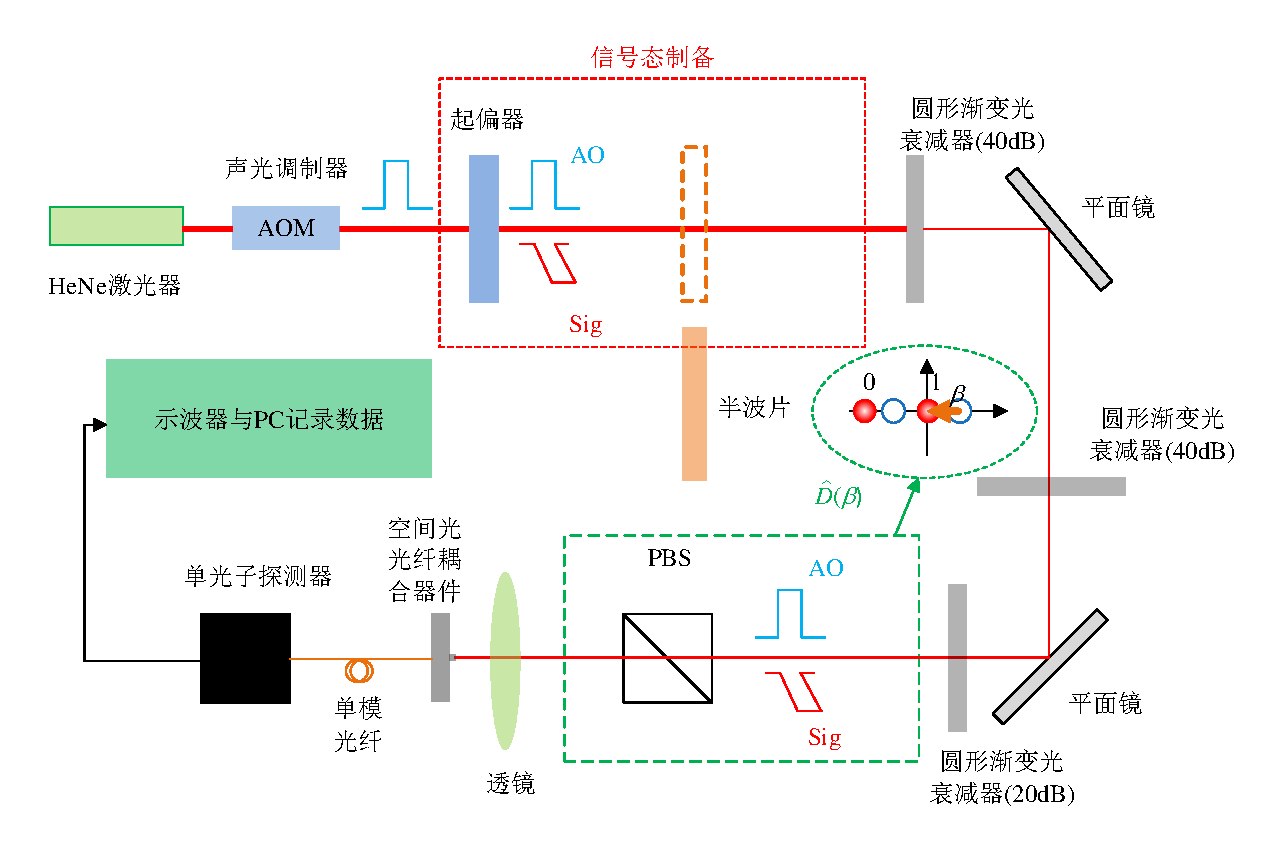
\includegraphics[width=\textwidth]{figures/chap5/Kennedy-receiver-diagram}
  \caption{Kennedy接收机实验光路示意图}
  \label{fig:Kennedy-receiver-diagram}
\end{figure}

实验光路示意图如图\ref{fig:Kennedy-receiver-diagram}所示,
实验照片如图\ref{fig:experiment-photo}所示。
线偏振的信号光通过一个半波片进行调制,
激光器采用JSDU公司生产的型号为1508P-2的氦氖激光器,
它输出0.5mW的632.8nm的线偏光,偏振度高达500:1。 
如果没有半波片意味着相移为$0$,
对应于符号$\ket{\alpha}$;
如果发送光路插入了半波片意味着相移为$\pi$,
对应于符号$\ket{-\alpha}$。
而在接收端,没有加半波片,
意味着位移操作为$\hat{D}(-\alpha)$。
实验光路取夹角为45°,因此系统效率最高为50\%。
通过采用一个偏振度高达1000:1的偏振分束器,
可以使得接收端最大光强与最小光强之比达到1:0.55\%,相当于条纹可见度为98.9\% 。
三个渐变衰减片组合后,提供最大到100dB的衰减量,
用以模拟深空光通信中的大损耗空间光路,对应到达接收端的光强水平为每个光脉冲中平均光子数单光子量级。
实验中取每个光脉冲宽度为5us,每次试验对符号$\ket{\alpha}$
和$\ket{-\alpha}$各重复$2\times 10^4$次。
在实验过程中,可以通过调节其中一个最大衰减系数为20dB的衰减片,
得到不同光强下的信号,
从而得到不同平均光子数下的平均错误概率。
最后进行光强探测的是Excelitas公司生产的型号为SPCM-AQRH16的单光子探测器。
该探测器在632.8nm光波长出的探测效率为65\%。初步实验中该探测效率和耦合损耗的可以计入空间光路损耗。
该探测器暗计数标称为25cps,实验当中由于环境杂散光等原因使得实际噪声光子计数比该数值要大。
实测的暗计数为35.9cps,因此一个光脉冲内的暗计数相当于$1.795\times 10^{-4}$个。
系统由于采用空间光路耦合,因此对环境光干扰很敏感,实验中将接收端
用遮光黑色纸盒减少环境光干扰和激光器的散射光干扰,
使环境光干扰降低至少10dB。


\begin{figure}
\centering
  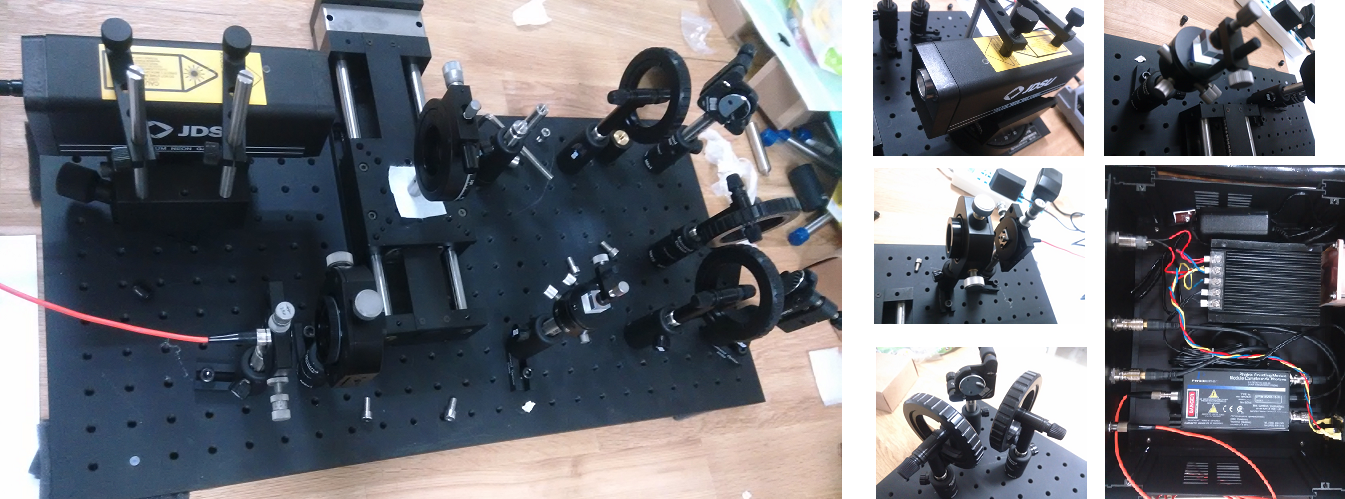
\includegraphics[width=\textwidth]{figures/chap5/experiment-photo}
  \caption{Kennedy接收机实验照片}
  \label{fig:experiment-photo}
\end{figure}

考虑到上述非理想环境下的条纹可见度和暗计数的情况下,
采用ON-OFF探测的Kennedy接收机平均错误概率为
\begin{equation}
P_e = \frac{1}{2}(1-e^{- 4 \eta |\alpha|^2 - v} + e^{- 2 \eta (1-\xi) |\alpha|^2 - v }).
\end{equation}
上式中,$\eta=50\%$为系统固有的效率,$\xi=98.9\%$是条纹可见度,$v=1.795\times 10^{-4}$是暗计数。

\begin{figure} %[H]
\centering
  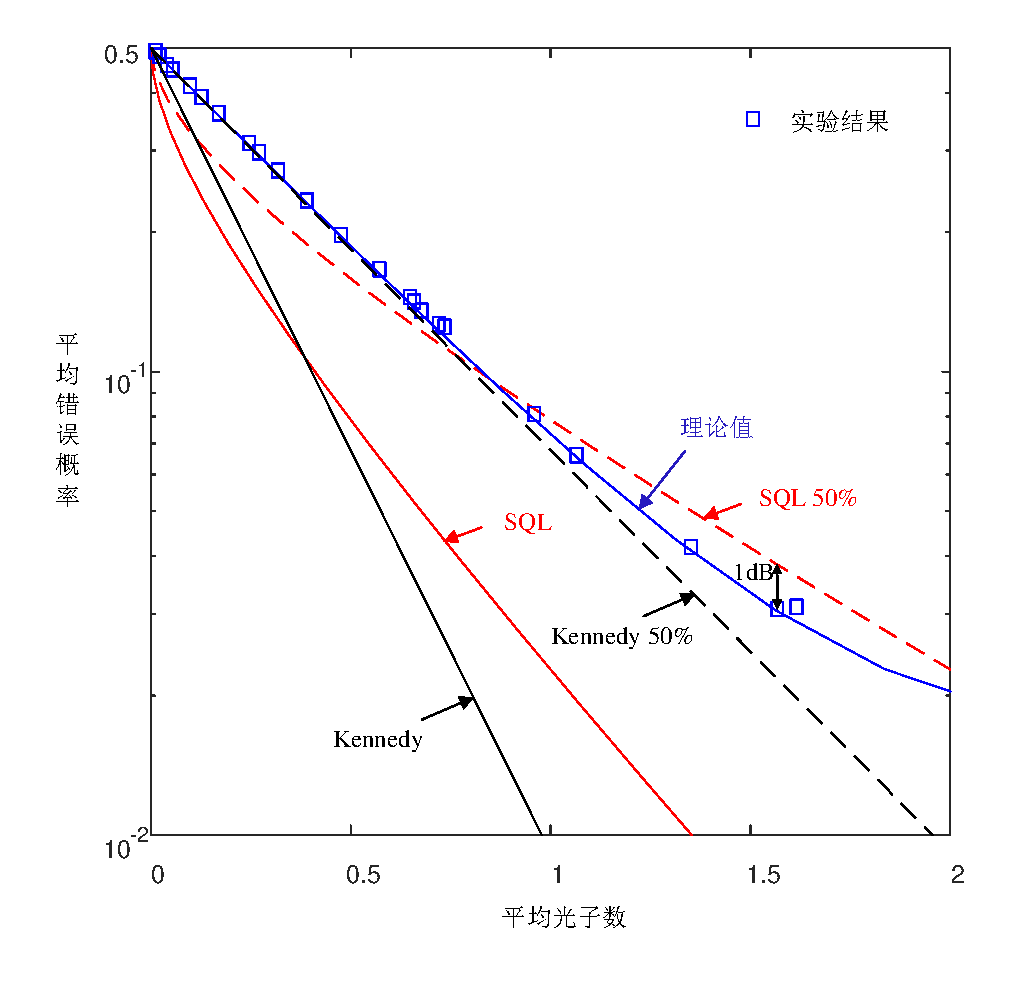
\includegraphics[width=0.6\textwidth]{figures/chap5/kennedy-experiment-error}
  \caption{Kennedy接收机实验结果}
  \label{fig:kennedy-experiment-error}
\end{figure}

\begin{table}
\caption{Kenendy接收机实验数据}
\label{tab:exp-data}
\centering
\begin{tabular}{cc}
\hline
每脉冲平均光子数 & 平均错误概率 \\
\hline
0.011 & 0.4898 \\ 
0.020 & 0.4814 \\ 
0.022 & 0.4791 \\ 
0.043 & 0.4604 \\ 
0.055 & 0.4499 \\ 
0.097 & 0.4153 \\ 
0.129 & 0.3898 \\ 
0.170 & 0.3604 \\ 
0.247 & 0.3099 \\ 
0.272 & 0.2969 \\ 
0.316 & 0.2728 \\ 
0.389 & 0.2345 \\ 
0.476 & 0.1975 \\ 
0.571 & 0.1659 \\ 
0.651 & 0.1444 \\ 
0.658 & 0.1418 \\ 
0.678 & 0.1355 \\ 
0.721 & 0.1269 \\ 
0.734 & 0.1252 \\ 
0.960 & 0.0815 \\ 
1.066 & 0.0662 \\ 
1.353 & 0.0417 \\ 
1.569 & 0.0309 \\ 
1.615 & 0.0312 \\ 
\hline
\end{tabular}
\end{table}


在实验过程中,通过改变可变衰减器的衰减值,
可以制备不同接收端接收光强下的相干光脉冲。
实验结果如图\ref{fig:kennedy-experiment-error}所示,
其中实验结果用方块表示出来,实验结果数据见表\ref{tab:exp-data},
理论计算值用蓝色实线标出,
可以看到,实验结果与理论值十分吻合。
我们还看到,虽然实验中的Kennedy接收机没能突破效率为1的标准量子极限(SQL),
但是突破了本系统固有效率为50\%的标准量子极限,最大的收益达到1dB。
因此,我们从实验上初步验证了在相同系统效率的情况下,
我们实验环境下的Kennedy接收机能够突破标准量子极限。


\section{总结}
在本章中,我们通过调研目前在实验室中实现的量子接收机实验方案,
并设计了自己的量子接收机试验方案。
通过对Kenendy接收机的实验,我们初步验证了这种实验方案的可行性。
这是国内首次从实验上证实量子接收机理论的先驱性工作。
在Kennedy接收机实验中,
我们的方案系统效率只有50\%,在后续的实验中,需要提升系统效率。
我们利用偏振器实现了98.9\%的条纹可见度,
但是与国外报告的实验方案相比,还是有较大差距。
Becerra团队利用相位稳定干涉仪实现了99.7\%的条纹可见度\cite{becerra2013experimental}。
而事实上,对接收机影响最大的非理想因素就是干涉的条纹可见度\cite{li2013suppressing}。
因此,有必要改进实验方案和器件,进一步提高干涉的条纹可见度。

从工程实现的角度来看,我们的实验方案和国际上现有的实现方案
中的本振都与信号同源\cite{wittmann2008demonstration,wittmann2010demonstration,tsujino2010sub,
tsujino2011quantum,becerra2011m,chen2012optical,muller2012quadrature,becerra2013experimental,
becerra2015photon}。我们实验当中使用的偏振复用的方案便于实现,
但是对光通信信道系统的偏振特性要求较高,难以应用到光纤链路当中。
而马赫曾德干涉仪的方案在发射端与接收端相距很远的时候难以保证
相位稳定,从而无法保证足够的条纹可见度。
因此如何实现高精度的光学相位跟踪和幅度跟踪成为工程上实现量子接收机
最关键的技术之一。




\chapter{总结与展望}
\section{研究成果总结}
在本论文研究内容的第一部分中,我们首先通过理论分析,
我们得到了QAM信号的标准量子极限和Helstrom极限的渐近性能分别为
$e^{-\alpha^2}$和$e^{-4\alpha^2}$,这里$\alpha$为相空间中,
符号间最小距离的一半,具体定义见第\ref{chp:qam}章。
由此可见如果采用最优量子检测方案,
接收机的性能将有指数倍的提升。
接着我们对Bondurant接收机、自适应分区检测接收机和混合接收机
等三类QAM信号量子接收机进行理论分析和数值仿真分析
我们发现这三类接收机都能突破标准量子极限,
且在较大信号时的理论渐近性能分析显示,这三种接收机比经典检测接收机的标准量子极限都有指数倍的收益。
相比较而言,自适应分区检测接收机最适合工程实现,
因为它只需要有限带宽的反馈控制即可,并且可以采用光子数可分辨的探测器减少分区数目并改善系统的鲁棒性。
QAM调制信号被广泛应用到大容量光通信中,
如果进一步采用量子接收机作为接收端,这将有利于进一步提升通信的信道容量,
进一步延长通信中继的距离。

在本论文研究工作的第二部分中,我们将目光从单个符号的检测放到多个符号的联合检测上来。
我们分析了OOK调制和BPSK调制下的多个符号联合检测问题,
这其中包括MPPM信号、编码后的OOK调制信号和编码后的BPSK调制信号。
首先我们通过理论分析,得出了这些信号的标准量子极限渐近性能为$e^{-\lceil d_{\min}/2\rceil \alpha^2}$,
而Helstrom极限大信号近似为$e^{-d_{\min} \alpha^2}$,这里$\alpha$为每个脉冲对应的复振幅,$d_{\min}$为最小码间距离,
详细定义见第\ref{chp:cpn}章。
接着采用Schmidt正交化的方法解决了他们的Helstrom极限数值求解问题。
最后,我们研究了针对这些调制信号的条件归零接收机的性能。
我们通过动态规划算法优化接收机的控制策略,
最终将接收机的误码率降低到经典检测方案的标准量子极限以下。
这种采用最优控制的条件归零接收机有望被应用到深空光通信中,
用来接收MPPM信号。这将极大地提高深空光通信的频谱利用率,从而进一步提高通信的信道容量。
针对二进制编码信号,这种联合监测方案将进一步降低误符号率,
能够进一步提高系统的能量效率。

在本论文研究工作的第三部分中,
我们设计了一个量子接收机实验方案,并从实验上初步验证了Kennedy接收机
的可行性。实验结果表明在我们的实验条件下,
Kenendy接收机可以突破相同系统效率的标准量子极限,最大增益达到1dB。
这为进一步的实验方案设计提供了实验经验的积累。
这种接收方案也有望应用到实际的自由空间深空光通信中,
将进一步降低误码率、提升通信系统的信道容量。

总的来说,本论文的创新点可以归纳如下:

1. 得到了QAM信号和编码后二进制调制信号的标准量子极限和Helstrom极限表达式。

2. 将Schmidt正交化应用到求解一般信号的Helstrom极限的问题当中,将求解算法复杂度降低。

3. 系统地研究了QAM信号三种量子接收机方案及其性能,证实了这三种方案都能突破标准量子极限,并且给出了工程应用的方案建议。

4. 系统地研究了MPPM信号和编码后二进制调制信号的条件归零接收机方案及其特性,将动态规划算法应用到接收策略优化当中,证实了使用条件归零接收机能够降低误码率,提升系统效率。


\section{研究工作展望}
在我们的研究过程中,
我们虽然解决了一些现有的问题,
但是仍然存在一些非常有价值的问题有待进一步研究。
对于QAM信号,我们可以将控制策略变为时变控制,
那么如何设计最佳的控制策略使得
接收机的误码率进一步接近Helstrom极限。
进一步,如何设计接收机对多元调制信号都能达到Helstrom极限。
对于联合检测方案,时变的最优控制策略仍然有待解决,
这种接收方案对极化编码能否逼近Holevo容量也是一个有待研究的问题。
最后,对于工程实现方面,如何在工程上实现精确的位移操作,
在本地实现高精度的光学相位和幅度跟踪是一个极大的挑战。
我们相信,未来的研究者在解决这些难题之后,
量子接收机应用到实际的光通信系统中将指日可待,
那时光通信的信道容量将得到进一步提升,
尤其是在能量受限和对能量效率要求很高的深空光通信中。




%\bibliographystyle{gbt7714-2005}
\bibliography{bib/tex}

%\appendix
%\chapter{论文规范}

\backmatter
\begin{acknowledgements}
光阴似箭,我的七年学习生涯转眼间就快结束了。
遥想当年刚进入科大时的意气风发,对未来的
学习生活充满憧憬。在这毕业之际,一时感慨万千。
首先,我要衷心感谢我的导师朱冰教授。自从
本科进入实验室开始,在这将近4年的时间里,
朱冰老师对我学习上和科研上给予了悉心的指导,
帮助我从科研的大门口开始了真正意义上的研究工作。
朱老师治学严谨、科研经历丰富,善于发掘本质问题,
常常一针见血指出科研中的问题。本论文的完成,从选题到
研究工作的完成过程,都离不开朱老师的细心指导。

感谢实验室杨利老师,她学术造诣深厚,为人亲切,
在研究生期间给予我亲切的鼓励。感谢实验室苏觉老师,
他对我的鼓励让我感受到实验室的人情味。

感谢实验室已毕业的李科师兄,在大四、研一和研二
期间,亲自带领我从量子接收机的入门课题开始,
到后续的深入研究。在整个过程中,
李科师兄总是不厌其烦地解答我研究中的问题。
即使在毕业之后,也不断的督促我和指导我的研究工作。
另外,我也要感谢已毕业的王晓飞师兄、许华醒师兄,
在实验室的时候给我的指导和帮助。

感谢研究生师兄陈林勋、朱圣强,与在实验室
与他们一起科研和生活的日子让我记忆深刻。
他们对学习的认真深刻地影响着我,在找工作期间
也作为过来人给予我细心的指导。

感谢博士师姐陈田,她科研的认真和永不放弃的毅力
给我留下深刻的印象。在科研和论文完成期间也
和她多番讨论,这些讨论给与我灵感和帮助。
感谢惠军和仇楠师弟,在实验室期间一直给与我实验上的帮助。

感谢实验室的师弟师妹们,与他们在一起的研究生生活,
让我感受到实验室的温馨。

感谢远在纽约的大学同学王洋,在我完成会议论文期间,
给予我英语上的帮助,感谢和我一起度过这七年时间的所有同学,
和他们一起学习,度过这七年的校园生活,让我倍感温馨。

感谢我的父母,没有他们的支持,我是不可能顺利完成学业的,
感谢我的女友对我学习的支持和鼓励。

感谢在学习期间所有帮助过和关心过我的父母、师长、同学和朋友,
在美好的校园生活即将结束之际,谨以此文献给我逝去的青春,
献给关心过我的你们!

\end{acknowledgements}

\begin{publications}

\section*{已发表论文}

\begin{enumerate}
\item Yuan Zuo, Tian Chen, Bing Zhu, "Conditional Pulse Nulling Receiver for Multi-pulse PPM and Binary Quantum Coding Signals", (ICWOC 2016, Beijing)
\item Yuan Zuo, Ke Li, Bing Zhu, "16-QAM Quantum Receiver with Hybrid Structure Outperforming the Standard Quantum Limit" , (APOP 2016, Shanghai)
\item Li K, Zuo Y, Zhu B. Suppressing the errors due to mode mismatch for M-ary PSK quantum receivers using photon-number-resolving detector[J]. IEEE Photonics Technology Letters, 2013, 25: 2182-2184.
\end{enumerate}



\end{publications}


\end{document}
